% ELEC5305 final report. Compile this file with pdfLaTeX or Tectonic.
% ELEC5305 research report source.
\documentclass[11pt,a4paper]{article}
\usepackage[margin=24mm,headheight=14pt]{geometry}
\usepackage[T1]{fontenc}
\usepackage{amsmath}
\usepackage{newtxtext,newtxmath}
\usepackage{microtype}
\usepackage{graphicx}
\usepackage{booktabs,tabularx,array}
\usepackage[table]{xcolor}
\usepackage{caption}
\usepackage{placeins,float}
\usepackage{fancyhdr,lastpage}
\usepackage{xurl}
\usepackage{hyperref}
\definecolor{navy}{HTML}{173B54}
\definecolor{tablegray}{HTML}{E9EEF2}
\hypersetup{colorlinks=true,linkcolor=navy,citecolor=navy,urlcolor=navy,
 pdftitle={Does a CNN Improve DSP-Based Ultrasonic Flaw Detection on Unseen Sources?},
 pdfauthor={Karthik Ramesh},pdfsubject={ELEC5305 Final Research Report},bookmarksnumbered=true}
\captionsetup{font=small,labelfont=bf,skip=7pt}
\captionsetup[table]{position=top}
\setlength{\parindent}{0pt}
\setlength{\parskip}{6pt plus 1pt}
\setlength{\emergencystretch}{2em}
\renewcommand{\arraystretch}{1.22}
\newcolumntype{Y}{>{\raggedright\arraybackslash}X}
\pagestyle{fancy}
\fancyhf{}
\fancyhead[L]{\small ELEC5305 Final Research Report}
\fancyhead[R]{\small Karthik Ramesh}
\fancyfoot[L]{\small SID 550754365}
\fancyfoot[R]{\small \thepage\ / \pageref*{LastPage}}
\renewcommand{\headrulewidth}{0.3pt}
\renewcommand{\footrulewidth}{0pt}
\raggedbottom
\clubpenalty=10000
\widowpenalty=10000
\setcounter{tocdepth}{2}
\begin{document}
\begin{center}
{\LARGE\bfseries Does a CNN Improve DSP-Based Ultrasonic Flaw Detection on Unseen Sources?\par}
\vspace{10pt}
{\large ELEC5305 Final Research Report\par}
\vspace{7pt}
{\large Karthik Ramesh\par}
{SID 550754365\par}
\end{center}
\vspace{5pt}
\textbf{GitHub code and reproducibility:}\\
\url{https://github.com/karthikramesh7512-cmd/elec5305-project-550754365}

\textbf{Demonstration video:}\\
\url{https://github.com/karthikramesh7512-cmd/elec5305-project-550754365/blob/main/docs/video/project_demo.mp4}
\vspace{7pt}
\section*{Abstract}

This study asks whether a compact convolutional classifier applied after a fixed ultrasonic DSP front end improves detection of previously unseen experimental flaw sources relative to a validation-thresholded DSP detector. Seven thousand experimental B-scans are evaluated with six frozen source-holdout folds; the ordinary image-level split is a reference. DSP cropping, per-A-scan DC removal and Hilbert-envelope extraction are shared, while the CNN learns from compressed envelope maps. Three fixed training seeds are evaluated without test-driven model selection. Across the six held-out sources, CNN macro recall is 85.07\% (seed SD 1.02 percentage points), compared with 66.67\% for DSP and 99.79\% for the SVM. CNN macro balanced accuracy is 92.54\% (seed SD 0.51 points), versus 83.33\% for DSP and 99.89\% for the SVM. The repeated no-flaw background and augmented positive images restrict the scope of these findings. Supplementary tests add frozen-model Gaussian-noise stress testing, simulation-trained transfer and measured full-matrix imaging. All simulation-trained methods score perfectly on the experimental target, but the domains share one identical negative image. The measured imaging pilot gives a 3.91 mm nominal-tip error after backwall calibration and does not establish reliable localisation. The contribution is a reproducible comparison and diagnosis of its limits, rather than industrial qualification.

\clearpage

\begingroup\small\setlength{\parskip}{0pt}\tableofcontents\endgroup

\clearpage

\FloatBarrier
\section{Introduction and research question}

Ultrasonic inspection identifies internal reflectors through the amplitude and spatial structure of returned signals. A practical automated detector must recognize flaw responses beyond the particular sources used for development. High accuracy on randomly partitioned augmented images may coexist with poor transfer to an unseen source. This makes the evaluation protocol part of the research question rather than a final reporting detail.

The single research question is: 	extbf{Does replacing the final deterministic DSP decision rule with a compact CNN improve ultrasonic flaw detection on previously unseen P41 source labels, using the same experimental data and frozen evaluation folds?} The SVM is an additional learned reference that helps distinguish an advantage over a simple threshold from an advantage specific to convolutional feature learning.

The reviewed ultrasonic studies link performance to flaw composition and inspection context \cite{ref1,ref2,ref5}. That motivates a bounded question about source transfer rather than treating random-split accuracy as evidence of general inspection capability.

This project contributes an image-identity audit, a frozen-source comparison with per-sample provenance, and a direct diagnosis of why score ranking and operating recall can diverge. Published methods motivate the experiment; the additional CNN and audit do not constitute a reproduction of those networks.

The first project stage established the dataset audit and DSP/SVM baselines. The final extension adds a compressed-envelope CNN, repeated-seed evaluation, saved inference demonstration and direct comparison. The primary scope is binary detection. Three supplementary studies now test controlled additive-noise sensitivity, simulation-trained transfer, and a separate measured-FMC imaging feasibility example. They probe boundaries of the main conclusion; they do not establish industrial qualification or equivalent crack sizing.

\FloatBarrier
\section{Literature review and conceptual background}

\subsection{Data diversity and source exclusion}

Virkkunen et al. \cite{ref1} combine B-scan CNN classification with virtual-flaw augmentation. Their blind human/network comparison uses 200 images, including 86 with cracks; however, the underlying raw data contain only three real cracks. The strength is an inspection-relevant comparison rather than image accuracy alone. Its limitation is that many augmented observations do not supply comparable physical-flaw diversity. This project consequently audits image identity and separates source labels; it does not reproduce their inspector comparison or probability-of-detection qualification.

Koskinen et al. \cite{ref2} test excluded flaw types after varying the training sources, measuring probability of detection (POD) and false calls. Their medium-flaw training case misses smaller indications. This motivates source-wise evaluation, while their different training combinations and POD endpoint prevent direct numerical comparison with this report.

The distinction is between generating more observations and representing more inspection conditions. Source separation addresses one dependence mechanism, but cannot repair the single negative background found in this dataset. A model can appear reliable because normal examples are unusually easy, even when its positive-source transfer remains weak.

\subsection{Representation learning and recent directions}

Cortes and Vapnik \cite{ref3} motivate the SVM's margin-based classifier, whereas LeCun et al. \cite{ref4} motivate local filters and weight sharing. The practical trade-off here is feature control versus representation flexibility: the SVM uses interpretable summaries; the CNN retains a compressed spatial map but must learn useful filters from limited source diversity. Neither theory guarantees superiority on these data.

Herve-Cote et al. \cite{ref5} generate sectoral PAUT scans from limited FMC acquisitions and report that incorporating median-scan inspection context improves CNN detection. This gives a relevant alternative to simply enlarging a classifier: provide information about geometry. However, sectoral-scan context is not available as an equivalent input here. Their result motivates a future context-aware comparison, not an unsupported claim that this map-only CNN reproduces their performance.

McKnight et al. \cite{ref6} use self-supervised forecasting on nominally sound CFRP data to identify anomalous regions and produce volumetric segmentation. They evaluate flat-bottom holes and PTFE inserts, including stepped geometries. This reduces dependence on labelled flaw examples and shifts the modelling problem toward learning normal structure. For this project, however, one repeated normal image is insufficient evidence for a realistic normal distribution. Different materials, tasks and metrics also prevent direct numerical comparison.

\begin{table}[H]
\centering
\caption{Selected literature and its implications for the experiment.}
\label{tab:1}
\small
\setlength{\tabcolsep}{4pt}
\begin{tabularx}{\linewidth}{@{}YYY@{}}
\toprule
\rowcolor{tablegray}
\textbf{Study} & \textbf{Approach and evaluation} & \textbf{Implication for this project} \\
\midrule
Virkkunen et al. \cite{ref1} & Virtual flaws; CNN; blind inspector comparison & Augmentation does not establish physical diversity \\
Koskinen et al. \cite{ref2} & Alter training sources; test excluded types & Evaluate small-source transfer explicitly \\
Herve-Cote et al. \cite{ref5} & FMC-derived sectoral scans with geometric context & Context is a competing route to better features \\
McKnight et al. \cite{ref6} & Sound-data forecasting; volumetric anomaly segmentation & Independent normal data are needed for this alternative \\
\bottomrule
\end{tabularx}
\end{table}

These selected 2021-2025 studies show two relevant research directions: improving the information presented to supervised models and reducing dependence on labelled flaws through anomaly modelling. Both remain constrained by representative acquisitions and evaluation design. The narrow gap addressed here is whether a lightweight envelope-map CNN improves the operating performance of an existing deterministic detector when positive source labels are excluded. It is a controlled local contribution, not an architectural state-of-the-art claim.

\subsection{Concepts needed to interpret the experiment}

The analytic signal combines an RF trace with its Hilbert transform; its magnitude gives an envelope that reduces dependence on the carrier phase. A CNN applies learned spatial filters, followed here by nonlinear activations and pooling. Binary cross entropy trains a logit, and the sigmoid maps that logit to a score between zero and one. That score is not assumed to be calibrated probability under source shift.

Recall is TP/(TP+FN), specificity is TN/(TN+FP), and balanced accuracy is their arithmetic mean. ROC-AUC describes ranking across thresholds; it does not guarantee good recall at a selected operating point. This distinction is essential because the saved DSP detector ranks each held-out source perfectly while missing both smaller sources at its validation-derived thresholds.

\subsection{Array imaging as a separate feasibility extension}

Holmes, Drinkwater and Wilcox \cite{ref8} describe retaining every transmitter-receiver waveform and focusing the array during post-processing. This motivates total focusing method (TFM) reconstruction as a transparent physics-based imaging reference. Its strength is explicit travel-time geometry; its weakness here is dependence on the velocity and time-origin model in a welded specimen. The public Strathclyde FMC dataset \cite{ref7} supplies measured array data and approximate flaw geometry for a small feasibility study. This imaging example uses different data and evaluates a different endpoint from the classifier comparison; it cannot show that the CNN localises flaws.

\FloatBarrier
\section{Methods}

\subsection{Data and integrity audit}

The study uses NDT\_ML\_Flaw experimental batches 013-019: 7,000 rows, including 3,442 positive and 3,558 negative rows. Raw images decode as little-endian int16 arrays of shape 480 by 7168. There are six recorded positive source labels. The 3,442 positive rows contain 1,880 distinct raw-image hashes; no identical positive hash spans multiple source labels. All negative rows contain one repeated image. These counts describe data identity, not proof of independence between distinct augmented images.

Each raw sample used for the CNN is checked against its original saved SHA-256 image hash. The 105 protected data/results files are checked before and after the new experiment. The baseline detector, saved SVMs, split manifests, labels and previous numerical results are neither regenerated nor altered.

\subsection{Frozen evaluation design}

The primary protocol contains six source-holdout folds. In each fold one source is tested, the next source cyclically is used for validation, and the remaining four sources train the model. Fixed negative groups of 593 rows rotate through the same roles. They are row groups, not independent negative acquisitions. A separate ordinary split uses 4,900 training, 1,050 validation and 1,050 test rows. It is reported only as an easier reference condition.

All methods are compared on exactly the same test sample IDs for each evaluation. CNN weights and normalization are fitted on training data only. Validation balanced accuracy chooses checkpoints, with lower validation loss breaking ties and the earliest epoch retained on an exact tie. All 21 selected checkpoints are saved and hashed before any CNN test evaluation. No test outcome changes the architecture, seed list, threshold or training budget.

\subsection{Deterministic DSP and SVM references}

The frozen DSP detector crops columns 1100:3100, removes each A-scan mean and computes the Hilbert envelope. It takes the maximum envelope response along each A-scan and smooths that spatial profile with candidate windows 1, 3, 5 and 7. Validation balanced accuracy selects a window and threshold; ties choose the highest optimal threshold and then the smallest window. Window 1 was selected in every saved evaluation. The final decision is score greater than or equal to threshold.

The saved SVM uses 12 engineered features including envelope amplitude statistics, RF RMS/energy, envelope energy, crest factor, peak counts, persistence, response width and spatial peak statistics. A training-only StandardScaler precedes the SVM. The original linear/RBF grid and validation selection are reused as historical evidence, without refitting. Comparing the CNN to this stronger reference guards against attributing every improvement over thresholding to deep learning.

The saved SVM search uses linear C in \{0.01, 0.1, 1, 10, 100\}, or RBF C in \{0.1, 1, 10, 100\} with gamma in \{scale, 0.001, 0.01, 0.1, 1\}. Validation balanced accuracy chooses the configuration; fixed grid order breaks ties. Training and validation are not combined for a refit. The 12 features and original fitting records remain documented in the saved SVM report.

\subsection{DSP plus CNN pipeline}

The DSP front end can be written compactly for scan line s and cropped sample t:

\begin{equation}x_c(s,t)=x(s,t)-\operatorname{mean}_{t}\!\left[x(s,t)\right]\end{equation}

\begin{equation}E(s,t)=\left|x_c(s,t)+j\,\mathcal{H}_{t}\!\left[x_c(s,t)\right]\right|\end{equation}

\begin{equation}M(i,k)=\log\!\left(1+\max_{\substack{0\leq a<8\\0\leq b<16}} E(8i+a,16k+b)\right)\end{equation}

Here H denotes the Hilbert transform along the time/depth axis. The deterministic detector reduces E to a maximum spatial response; the CNN retains a coarse two-dimensional map M. For each evaluation, the CNN input is \( (M-\mu_{\mathrm{train}})/\sigma_{\mathrm{train}} \), using one scalar mean and standard deviation fitted on training maps only. Its output logit z is converted to \(p=1/(1+\exp(-z))\); the frozen rule is \(z\geq 0\), equivalently \(p\geq 0.5\). A high ranking AUC does not require that a useful boundary coincides with zero.

\begin{figure}[H]
\centering
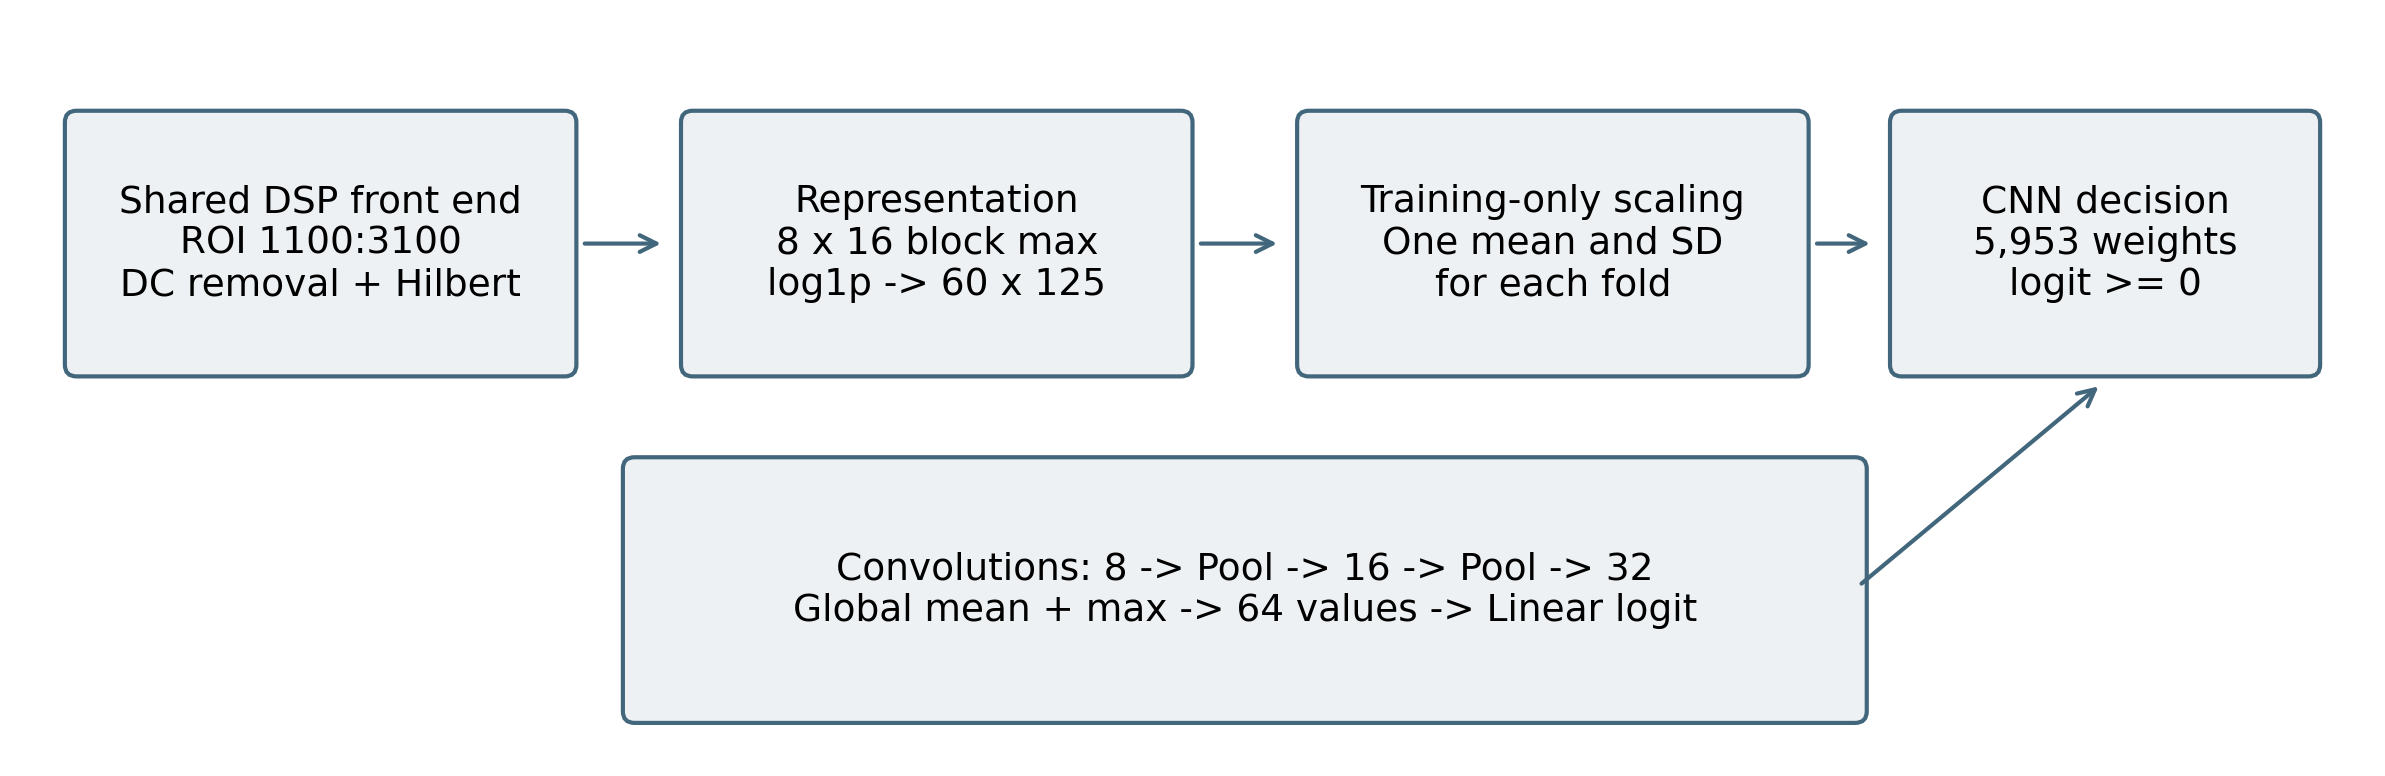
\includegraphics[width=\linewidth,height=0.42\textheight,keepaspectratio]{figures/figure_01.png}
\caption{Shared DSP preprocessing and the added CNN representation and decision stages. No source label or flaw annotation enters the network.}
\label{fig:1}
\end{figure}

The CNN shares the same crop, DC removal and Hilbert magnitude. Non-overlapping 8 by 16 block maxima compress the 480 by 2000 envelope to 60 by 125. Fixed log1p compression reduces its dynamic range. Maximum pooling retains local peaks efficiently, but can suppress fine morphology. A scalar mean and standard deviation are estimated from training maps separately in each fold; no validation or test inputs contribute to these fitted values. Source, size, location, depth and labels are excluded from the network input.

Three padded 3 by 3 convolutions use 8, 16 and 32 output channels, each with ReLU. The first two convolutions are followed by 2 by 2 maximum pooling. Global spatial means and maxima are concatenated and mapped to one logit. There are 5,953 trainable parameters. This is a learned detector on compressed DSP outputs, not an end-to-end RF model or a reproduction of the published ultrasonic networks.

Adam uses learning rate 0.001, weight decay 0.0001 and batch size 64 with unweighted binary cross entropy. The fixed budget is 20 epochs and patience is five epochs without improvement under the checkpoint ordering. Seeds 42, 43 and 44 are all reported; the best test seed is not selected. No additional augmentation or pretrained weights are used. The decision threshold is fixed at 0.5 sigmoid score. Training uses PyTorch 2.9.0+cu126 and an NVIDIA RTX 3060 Laptop GPU with deterministic algorithms enabled.

\subsection{Architecture and design rationale}

\begin{table}[H]
\centering
\caption{Compact CNN architecture and trainable parameter counts.}
\label{tab:2}
\small
\setlength{\tabcolsep}{4pt}
\begin{tabularx}{\linewidth}{@{}YYY@{}}
\toprule
\rowcolor{tablegray}
\textbf{Stage} & \textbf{Output excluding batch axis} & \textbf{Parameters} \\
\midrule
DSP map and training scaling & 1 x 60 x 125 & 0 fitted network weights \\
Conv 3 x 3 then ReLU & 8 x 60 x 125 & 80 \\
MaxPool 2 x 2 & 8 x 30 x 62 & 0 \\
Conv 3 x 3 then ReLU & 16 x 30 x 62 & 1,168 \\
MaxPool 2 x 2 & 16 x 15 x 31 & 0 \\
Conv 3 x 3 then ReLU & 32 x 15 x 31 & 4,640 \\
Global average and maximum concatenation & 64 & 0 \\
Linear logit & 1 & 65 \\
Total & Binary detection score & 5,953 \\
\bottomrule
\end{tabularx}
\end{table}

Block maxima reduce the map from 960,000 to 7,500 values, a 128-fold reduction, while retaining the strongest envelope sample in each block. This is motivated by echo detectability and memory efficiency, rather than proof that 8 by 16 is optimal. Its cost is loss of within-block morphology and position. Fixed log1p compression moderates amplitude range without dividing every image by its own maximum, which would remove absolute amplitude information that may aid detection.

Three small convolution layers offer hierarchical local filtering with a modest parameter count. The 3 by 3 filters encode a local-pattern assumption; pooling reduces spatial resolution and permits some positional tolerance. Global average pooling summarizes distributed responses, while global maximum pooling retains strong local responses. Concatenating them limits reliance on either statistic alone. The small linear head avoids a large position-specific dense layer. These are engineering rationales, not conclusions from an architecture search or feature-importance study.

The learning rate, weight decay, 20-epoch cap and patience of five were fixed practical choices for a compact, deadline-bounded experiment. They were not demonstrated to be optimal. Early stopping and three seeds provide limited checks on training behaviour but do not replace a validation-based configuration search. Binary cross entropy is \(\mathcal{L}=-\operatorname{mean}[y\log p+(1-y)\log(1-p)]\); equal class weighting is used because the row classes are approximately balanced, not because physical acquisition frequencies are known.

\subsection{Intended coverage and verification}

The intended comparison measures source-wise detection, ordinary-split reference performance, training variability and computational burden. Every seed reports confusion counts, accuracy, recall, precision, F1, specificity, balanced accuracy and ROC-AUC. Macro averages weight each held-out source equally; seed standard deviations describe training variation, not uncertainty across independent specimens. Per-sample outputs and full-precision tables accompany rounded report values.

Independent saved-result checks verify test coverage, labels, decisions, ROC-AUC, confusion counts, training/validation membership, checkpoint selection and baseline preservation. The short demonstration loads saved weights and fixed examples without retraining. Generalisation to new backgrounds would require additional independent acquisitions. The supplementary protocols below extend coverage without altering any original model, split or result. Independent physical no-flaw acquisitions remain unavailable; synthetic noise does not supply them.

\subsection{Frozen-model additive-noise stress test}

Additive white Gaussian noise is applied to the DC-centred 480 by 2000 RF region before envelope extraction, at ROI RMS SNR values of 20, 15, 10, 5 and 0 dB. For centred signal x and noise n, \(\mathrm{SNR}_{\mathrm{dB}}=20\log_{10}\!\left(\operatorname{RMS}(x)/\operatorname{RMS}(n)\right)\). Each noise field has its per-A-scan mean removed and is scaled to the requested SNR. Replicate seeds are 101, 102 and 103. Identical raw-image hashes receive identical noise within a replicate, so copied backgrounds do not become artificially independent observations. The same base Gaussian field is scaled across SNR conditions, yielding paired perturbations. SNR is relative to the complete centred ROI, not the unknown flaw-only response.

The six original DSP detectors and 18 source-holdout CNN checkpoints are reused with their original normalisation and decisions. No retraining or threshold adjustment occurs. The SVM is not included in this stress test. GPU Hilbert/map outputs are checked against the clean CPU representation with absolute tolerance 2e-6 before noise evaluation. The 360 saved rows cover six folds, five SNR values, three noise draws and four method/seed combinations. Macro metrics average the six sources; plotted standard deviations describe three DSP noise draws or nine CNN noise/initialisation combinations, not independent-acquisition confidence intervals. Gaussian injection does not model coupling changes, coherent weld clutter or instrument drift.

\subsection{Simulation-trained experimental-target transfer}

Ten local NDT\_ML\_Flaw simulated batches, 201-210, decode as 10,000 images with 5,018 positive and 4,982 negative rows. Batches 201-207 train the models, batch 208 selects configurations/checkpoints and batches 209-210 form a 2,000-row simulated reference test. All 7,000 experimental rows are the target, with no experimental-target fitting, validation or threshold selection. Simulation size codes are not mapped to millimetres because their physical encoding remains unverified. The same DSP candidates, 25-configuration SVM grid and single CNN configuration with all three seeds are fitted in a new results directory. All selections are frozen before reference-test and target evaluation. Original experimental models are preserved.

The pre-fit hash audit discovers exactly one identical image across the two domains: all 4,982 simulated negatives and all 3,558 experimental negatives share it. No positive raw hash overlaps. This discovery is disclosed before model fitting. The study therefore tests synthetic-positive to experimental-positive transfer on a shared normal background, not a fully independent simulated-to-real inspection domain. Experimental target specificity is particularly optimistic. Source and target positives may still be related through the upstream augmentation process; distinct hashes do not establish independent physical acquisitions.

\subsection{Measured FMC/TFM feasibility and independent backwall calibration}

The separately sourced Strathclyde dataset \cite{ref7} contains a measured welded 316L stainless-steel inspection, nominally a 6 mm lack-of-fusion flaw at 50 degrees. Acquisition metadata specify 128 elements at 0.7 mm pitch, 5 MHz nominal centre frequency, 100 MHz sampling, a 22 mm plate and longitudinal speed 5,820 m/s. The MATLAB variable FMC\_new actually has dimensions 10,000 by 128 by 128 (time, transmitter, receiver), correcting the order stated in the accompanying metadata. The raw file SHA-256, licence and download locations are saved in the repository.

After trace DC removal, a fourth-order 2-8 MHz Butterworth bandpass is applied with zero-phase filtering. Polyphase decimation by five gives a 20 MHz signal. Full-aperture TFM sums linearly interpolated analytic signals at each transmit-plus-receive propagation delay, using straight longitudinal rays and one homogeneous velocity. For grid point r, \[ I(\mathbf r)=\left|\sum_{\mathrm{tx},\mathrm{rx}}a_{\mathrm{tx},\mathrm{rx}}\!\left(\frac{\lVert\mathbf r-\mathbf r_{\mathrm{tx}}\rVert+\lVert\mathbf r-\mathbf r_{\mathrm{rx}}\rVert}{c}-t_0\right)\right|. \] The imaging grid spans x=0-90 mm and depth=1-26 mm at 0.25 mm spacing. A synthetic point-target test checks delay geometry and interpolation, but cannot validate the weld propagation approximation.

An initial reconstruction uses t0=0. Its backwall position motivates a separately saved calibrated variant. For diagonal pulse-echo traces from remote elements (x less than 20 mm or greater than 70 mm), the envelope peak is found in a predefined 4.5-10.5 microsecond window. The offset is expected backwall arrival 2h/c minus median observed arrival, giving t0=1.21014 microseconds. The nominal crack-tip position is not used to fit this calibration. Both reconstructions are retained.

For a bounded localisation check, the brightest amplitude is extracted from the metadata-assisted lower-tip ROI x=29-41 mm, depth=17-21.5 mm and compared with the approximate metadata point (35,20) mm. This is not blind localisation, and nominal-point distance is not metrologically established sizing error. The one-velocity model, approximate geometry, ROI selection and boundary peaks constrain interpretation. This pilot answers whether the imaging code executes on measured FMC data; it does not extend the CNN detector into a validated localiser.

\FloatBarrier
\section{Results}

\subsection{Primary source-holdout comparison}

\begin{table}[H]
\centering
\caption{Primary source-holdout comparison. CNN values are three-seed means and sample standard deviations.}
\label{tab:3}
\footnotesize
\setlength{\tabcolsep}{4pt}
\begin{tabularx}{\linewidth}{@{}YYYYYYY@{}}
\toprule
\rowcolor{tablegray}
\textbf{Source} & \textbf{Size mm} & \textbf{DSP recall \%} & \textbf{SVM recall \%} & \textbf{CNN recall \%} & \textbf{CNN BA \%} & \textbf{CNN AUC} \\
\midrule
P41\_01 & 2 & 0.00 & 98.72 & 10.42 \(\pm\) 6.14 & 55.21 \(\pm\) 3.07 & 1.0000 \\
P41\_02 & 3 & 0.00 & 100.00 & 100.00 \(\pm\) 0.00 & 100.00 \(\pm\) 0.00 & 1.0000 \\
P41\_03 & 26 & 100.00 & 100.00 & 100.00 \(\pm\) 0.00 & 100.00 \(\pm\) 0.00 & 1.0000 \\
P41\_04 & 6 & 100.00 & 100.00 & 100.00 \(\pm\) 0.00 & 100.00 \(\pm\) 0.00 & 1.0000 \\
P41\_05 & 17 & 100.00 & 100.00 & 100.00 \(\pm\) 0.00 & 100.00 \(\pm\) 0.00 & 1.0000 \\
P41\_06\_notch & 6 notch & 100.00 & 100.00 & 100.00 \(\pm\) 0.00 & 100.00 \(\pm\) 0.00 & 1.0000 \\
\bottomrule
\end{tabularx}
\end{table}

CNN values are mean \(\pm\) sample standard deviation across three seeds. DSP and SVM values are the preserved single-fit results. BA denotes balanced accuracy. AUC is the mean CNN ROC-AUC across seeds.

Across the six held-out sources, CNN macro recall is 85.07\% (seed SD 1.02 percentage points), compared with 66.67\% for DSP and 99.79\% for the SVM. CNN macro balanced accuracy is 92.54\% (seed SD 0.51 points), versus 83.33\% for DSP and 99.89\% for the SVM. For P41\_01, CNN recall is 10.42\% \(\pm\) 6.14 percentage points across seeds. For P41\_02, CNN recall is 100.00\% \(\pm\) 0.00 percentage points across seeds. Source-specific results must be inspected alongside these macro averages because a strong aggregate can conceal poor recall on the smallest source.

\begin{figure}[H]
\centering
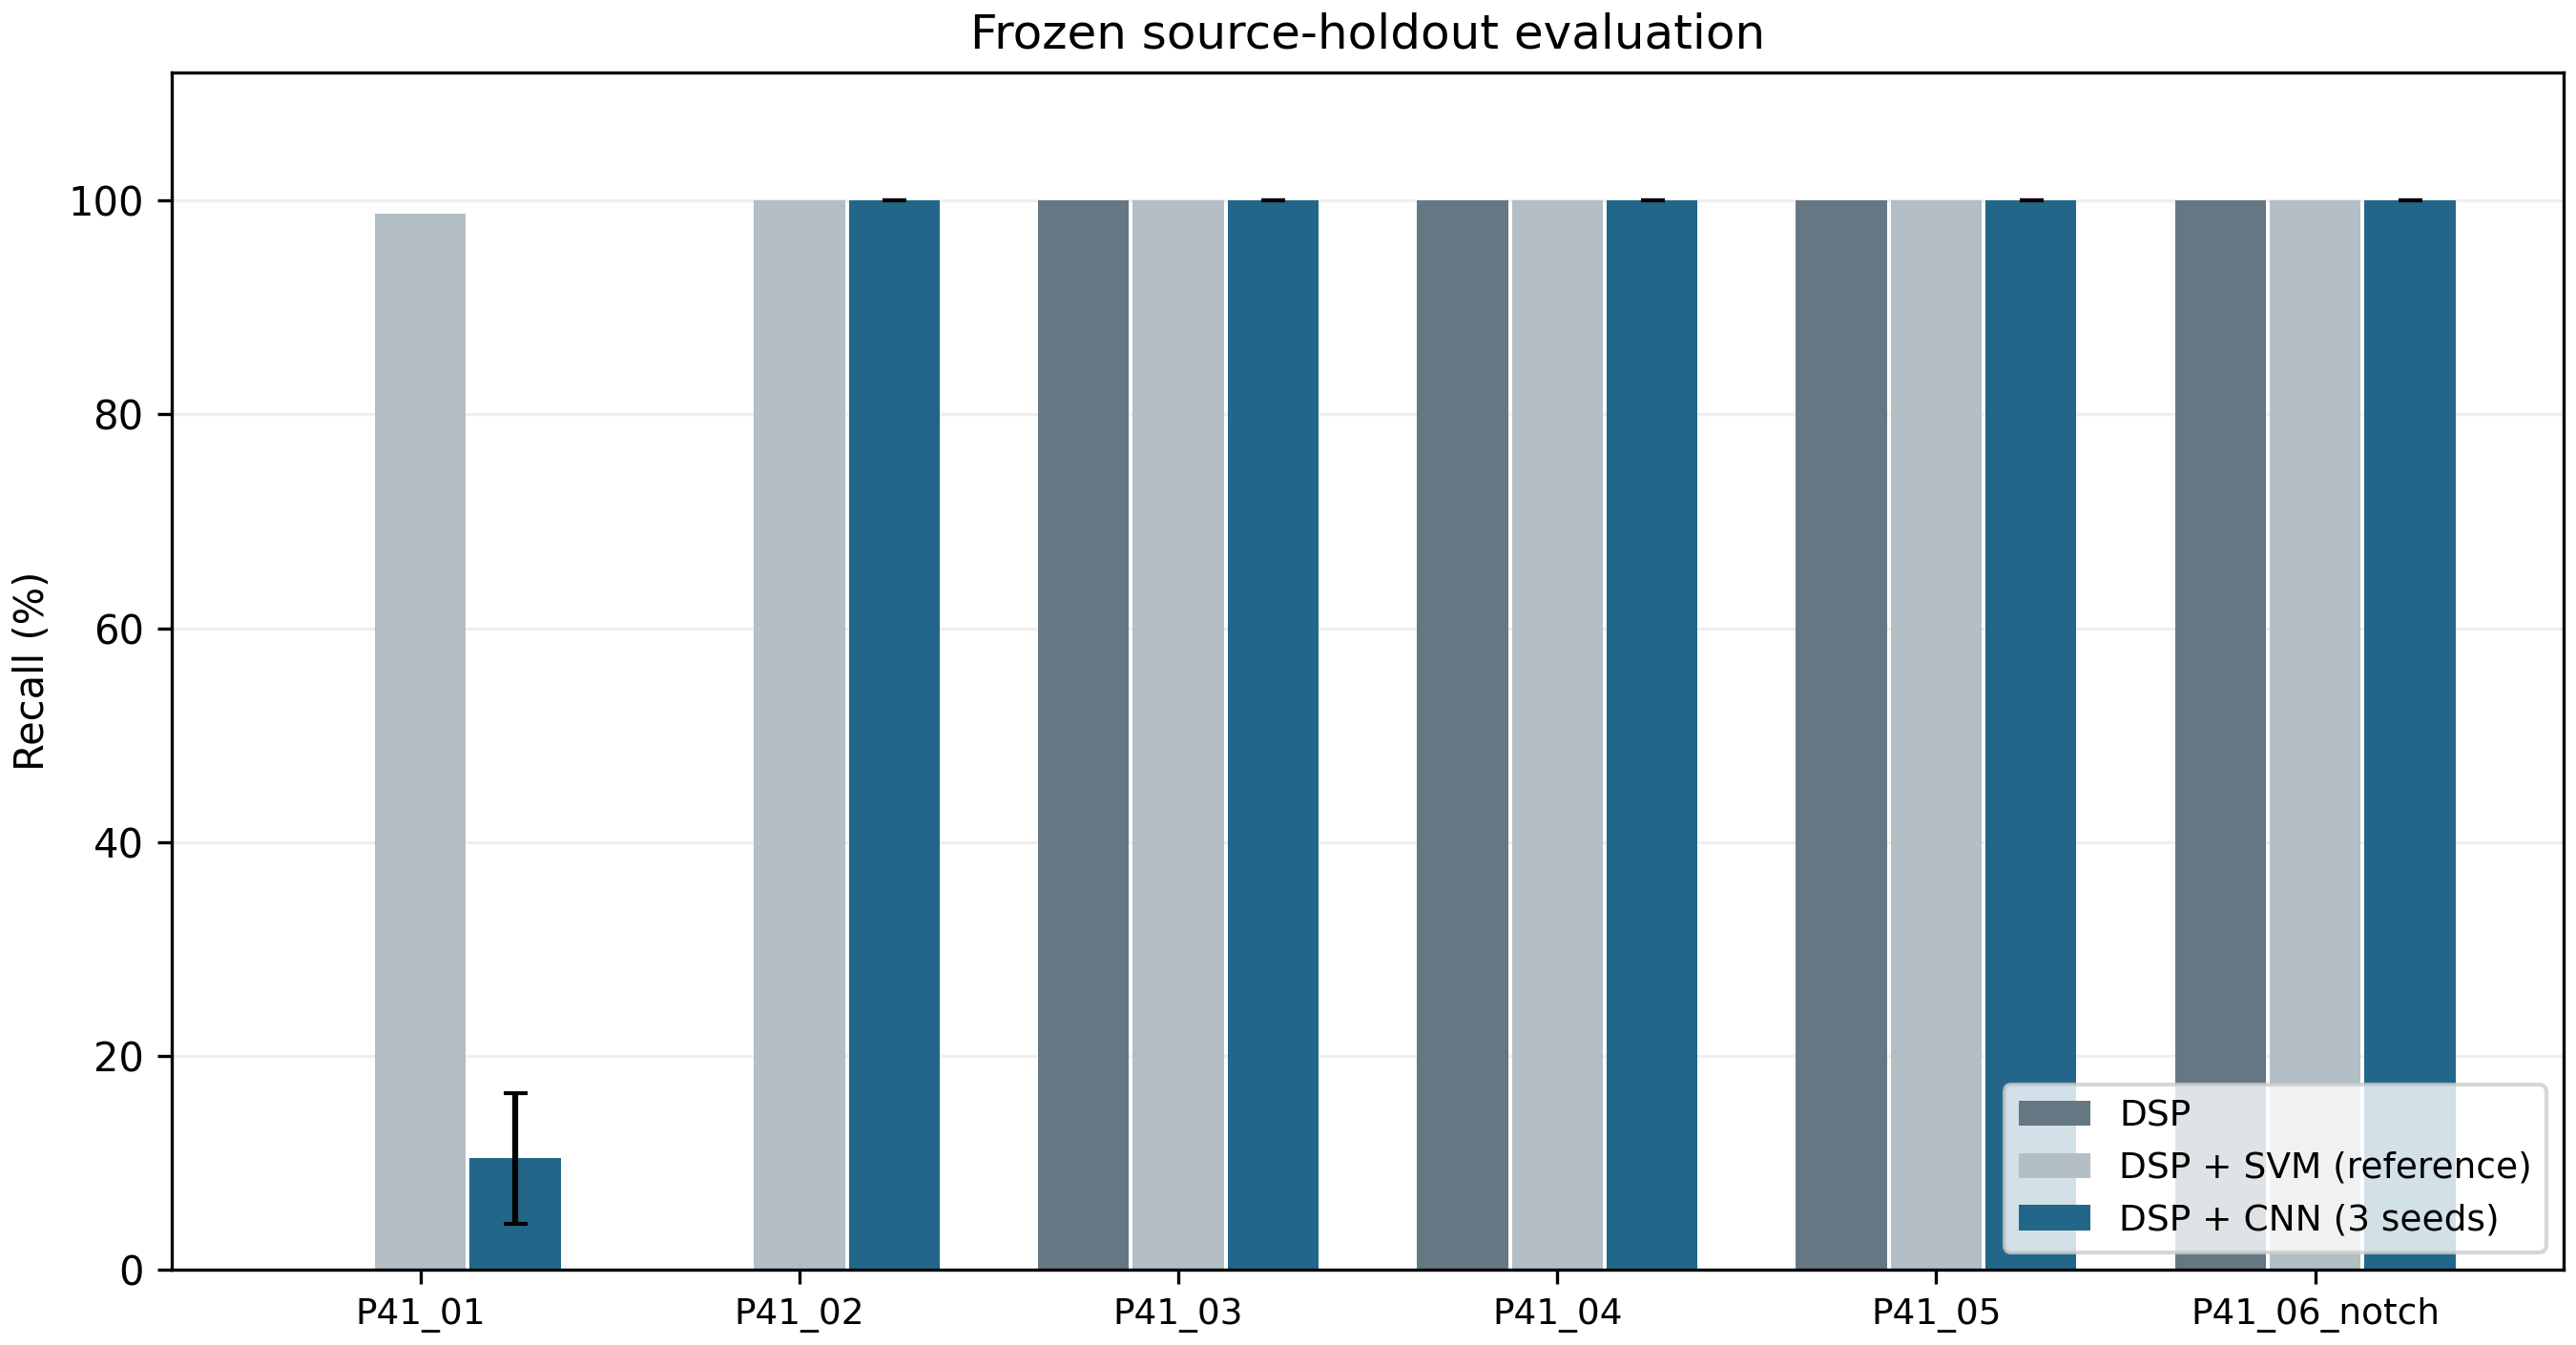
\includegraphics[width=\linewidth,height=0.42\textheight,keepaspectratio]{figures/figure_02.png}
\caption{Source-wise recall for the frozen DSP detector saved SVM and DSP plus CNN. CNN bars show seed means and error bars show seed standard deviation.}
\label{fig:2}
\end{figure}

\begin{figure}[H]
\centering
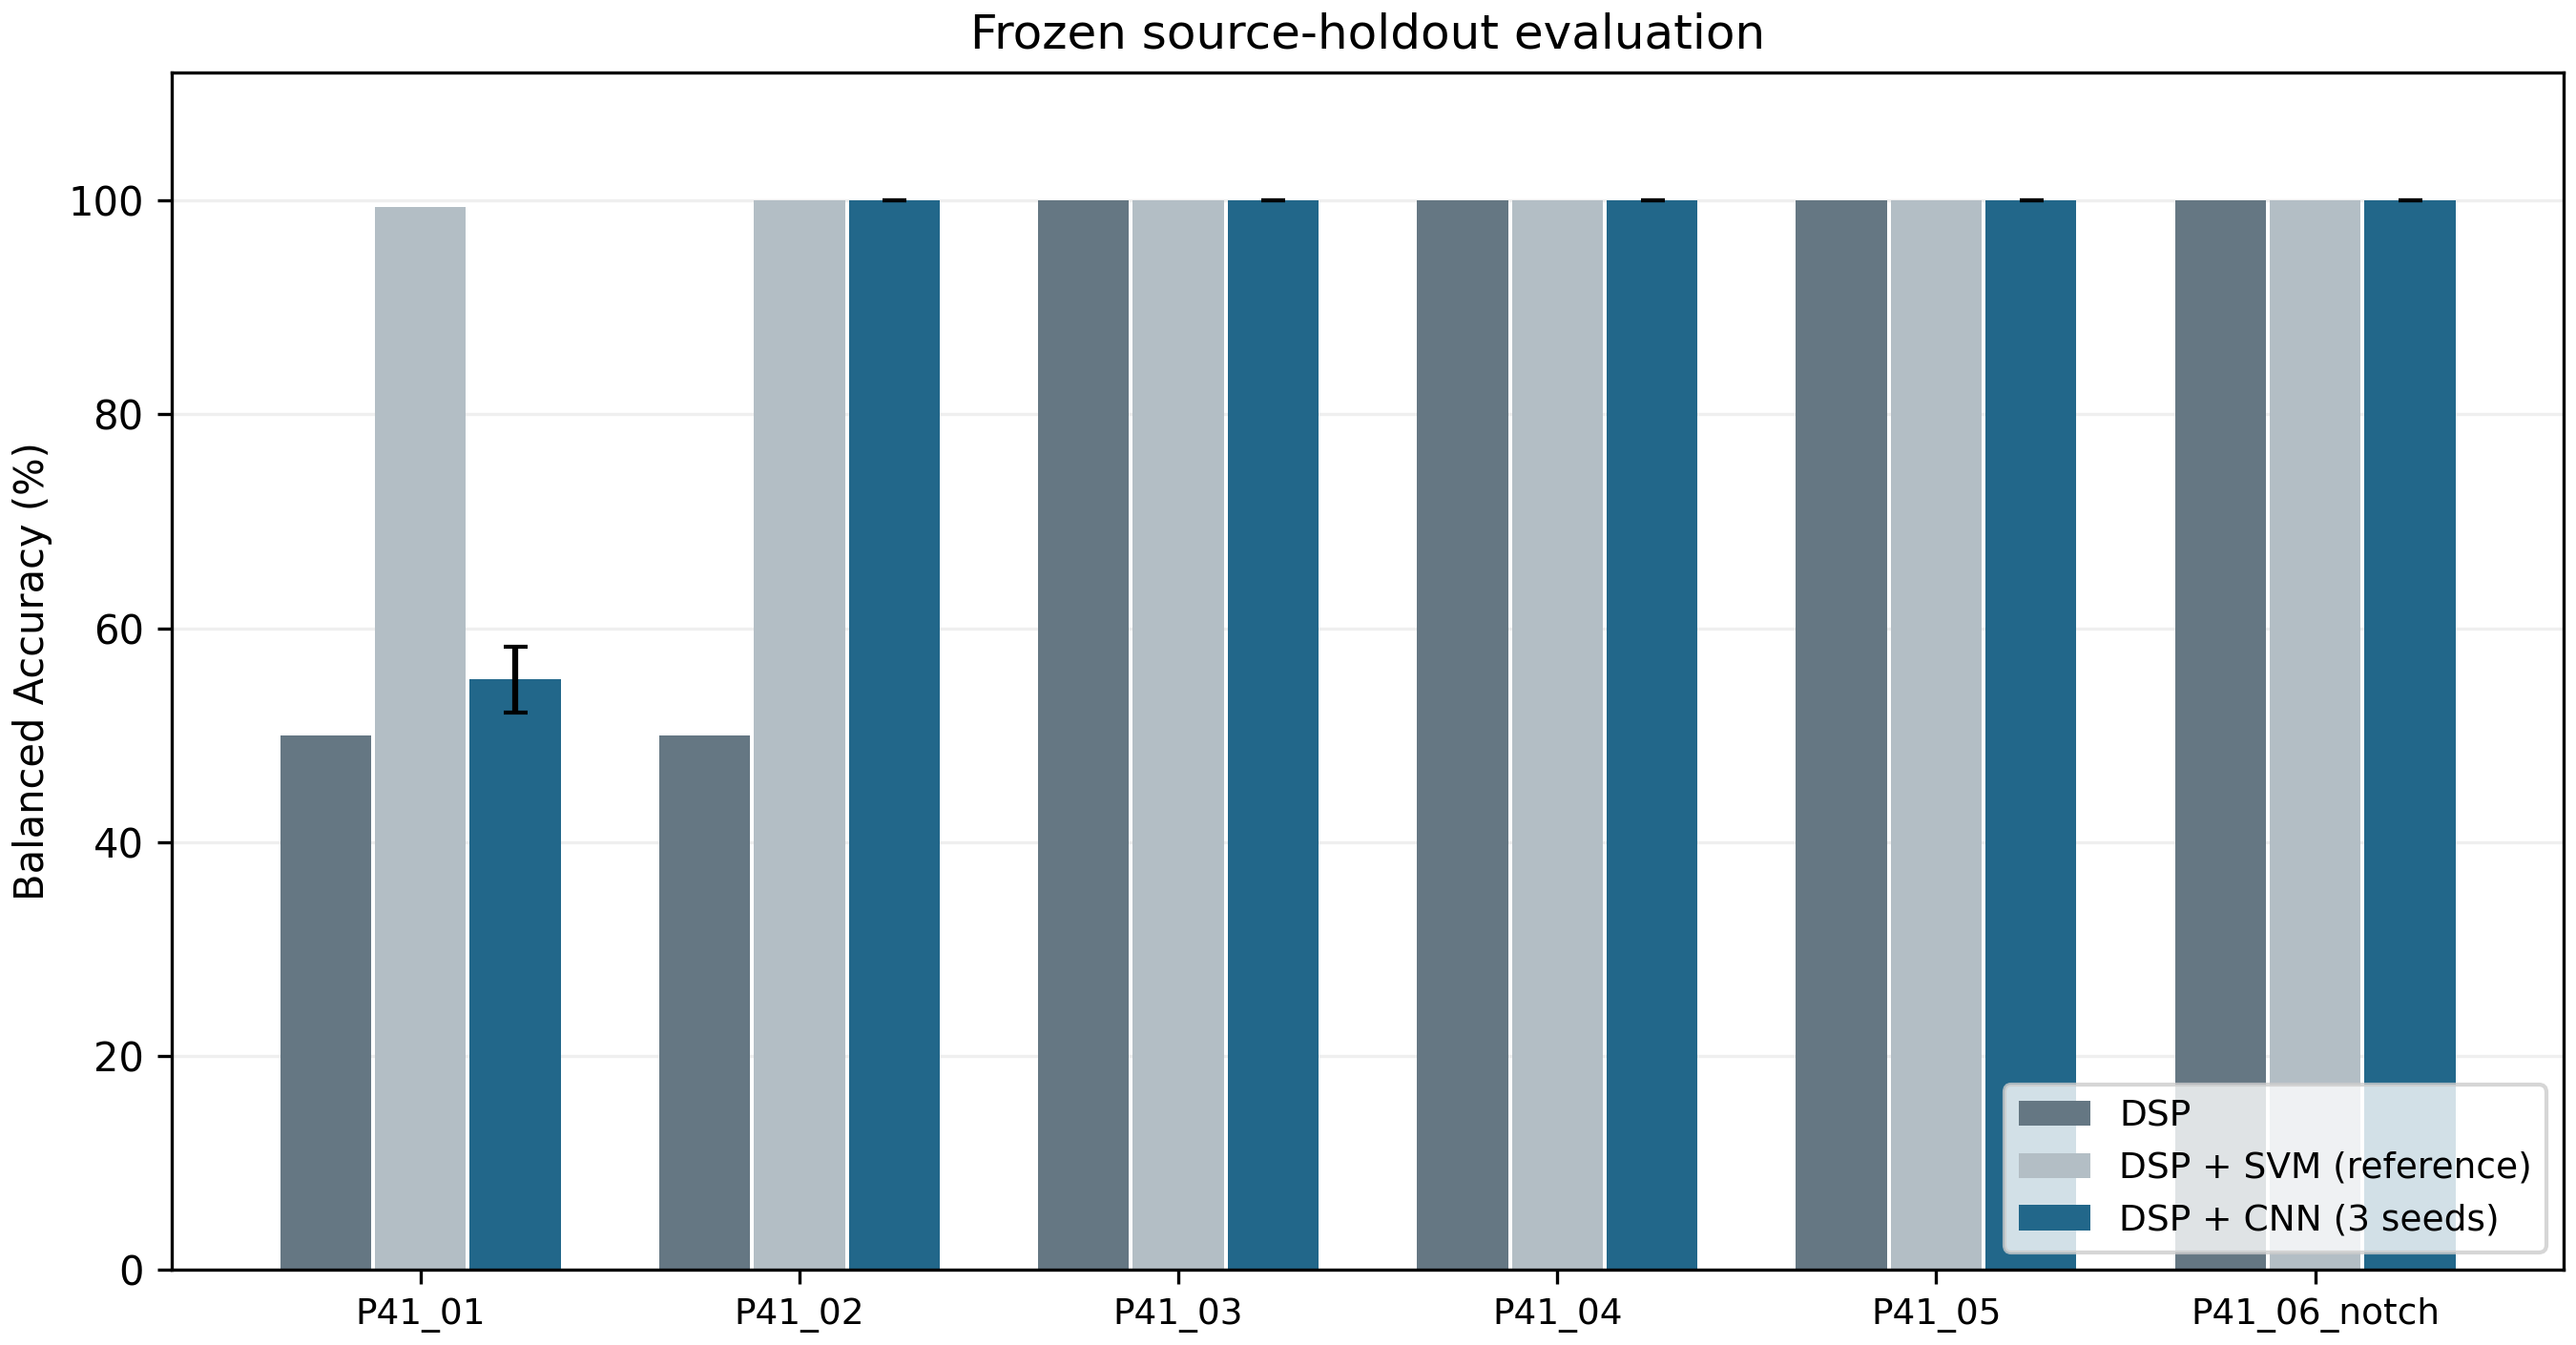
\includegraphics[width=\linewidth,height=0.42\textheight,keepaspectratio]{figures/figure_03.png}
\caption{Balanced accuracy for the same source-holdout test rows. High specificity is limited to one repeated negative background.}
\label{fig:3}
\end{figure}

\subsection{Direct evidence of operating-point transfer}

The following plot uses only saved fold-1 test logits, without rerunning inference. For each seed, every 2 mm positive logit exceeds every negative logit, consistent with ROC-AUC 1.0. Nevertheless, most positive logits remain below the frozen zero boundary. Thus the failure is visible in the score geometry: rank separation is preserved while the chosen operating point rejects most small-flaw rows. The plot diagnoses this saved result; it is not used to choose a replacement threshold.

\begin{figure}[H]
\centering
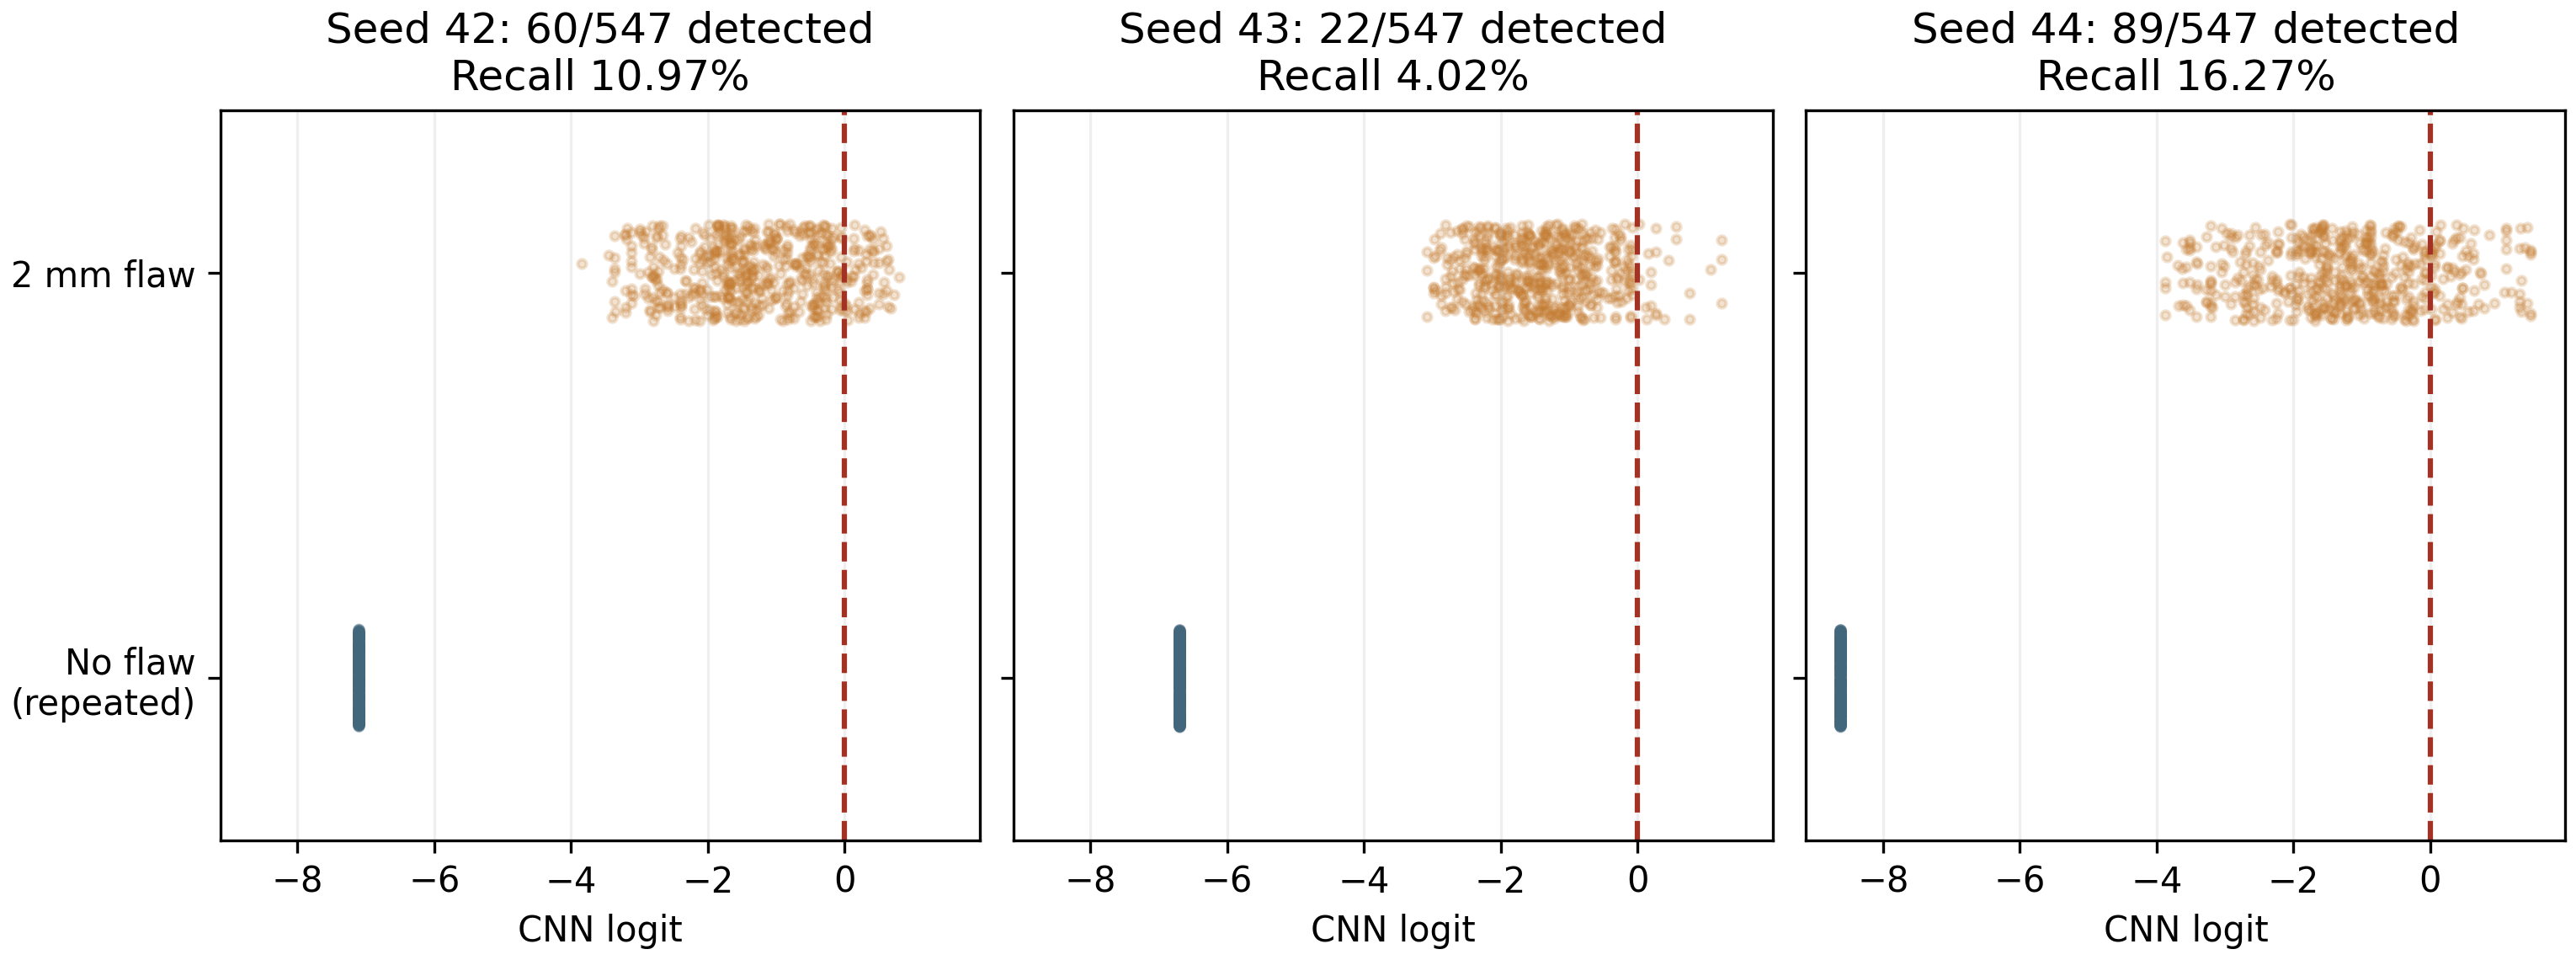
\includegraphics[width=\linewidth,height=0.42\textheight,keepaspectratio]{figures/figure_04.png}
\caption{Saved CNN logits for the held-out 2 mm source and repeated negatives. Horizontal positions are actual scores; seeded vertical jitter separates overlapping markers for visibility. The dashed line is the unchanged logit threshold of zero. Negative markers represent repeated rows of one background, not independent acquisitions.}
\label{fig:4}
\end{figure}

\subsection{Confusion counts and ordinary reference}

Across source-holdout folds, each seed evaluates all 7,000 rows once. The pooled confusion counts below weight rows rather than sources, so they answer a different aggregation question from macro recall.

\begin{table}[H]
\centering
\caption{Pooled CNN confusion counts across the six held-out sources, by training seed.}
\label{tab:4}
\small
\setlength{\tabcolsep}{4pt}
\begin{tabularx}{\linewidth}{@{}YYYYY@{}}
\toprule
\rowcolor{tablegray}
\textbf{Seed} & \textbf{TP} & \textbf{TN} & \textbf{FP} & \textbf{FN} \\
\midrule
42 & 2955 & 3558 & 0 & 487 \\
43 & 2917 & 3558 & 0 & 525 \\
44 & 2984 & 3558 & 0 & 458 \\
\bottomrule
\end{tabularx}
\end{table}

The ordinary split gives the following CNN reference results. Both saved DSP and SVM ordinary tests achieved 100\% accuracy and recall. Near-ceiling ordinary performance should not be substituted for the held-out-source comparison.

\begin{table}[H]
\centering
\caption{Ordinary image-level reference performance by CNN seed.}
\label{tab:5}
\small
\setlength{\tabcolsep}{4pt}
\begin{tabularx}{\linewidth}{@{}YYYYY@{}}
\toprule
\rowcolor{tablegray}
\textbf{Seed} & \textbf{Accuracy \%} & \textbf{Recall \%} & \textbf{Balanced accuracy \%} & \textbf{ROC-AUC} \\
\midrule
42 & 100.00 & 100.00 & 100.00 & 1.0000 \\
43 & 100.00 & 100.00 & 100.00 & 1.0000 \\
44 & 100.00 & 100.00 & 100.00 & 1.0000 \\
\bottomrule
\end{tabularx}
\end{table}

\subsection{Training behaviour and computational burden}

Selected epochs range from 3 to 20. Recorded training time totals 2.66 minutes across 21 fits, with median 8.35 seconds per fit on the stated GPU. This excludes decompression, preprocessing, cache generation and test inference. The parameter count is small, but CNN training and map generation introduce costs absent from the frozen threshold detector. No matched end-to-end timing benchmark was conducted, so these numbers do not establish deployment throughput or fair latency ratios against DSP/SVM.

\begin{figure}[H]
\centering
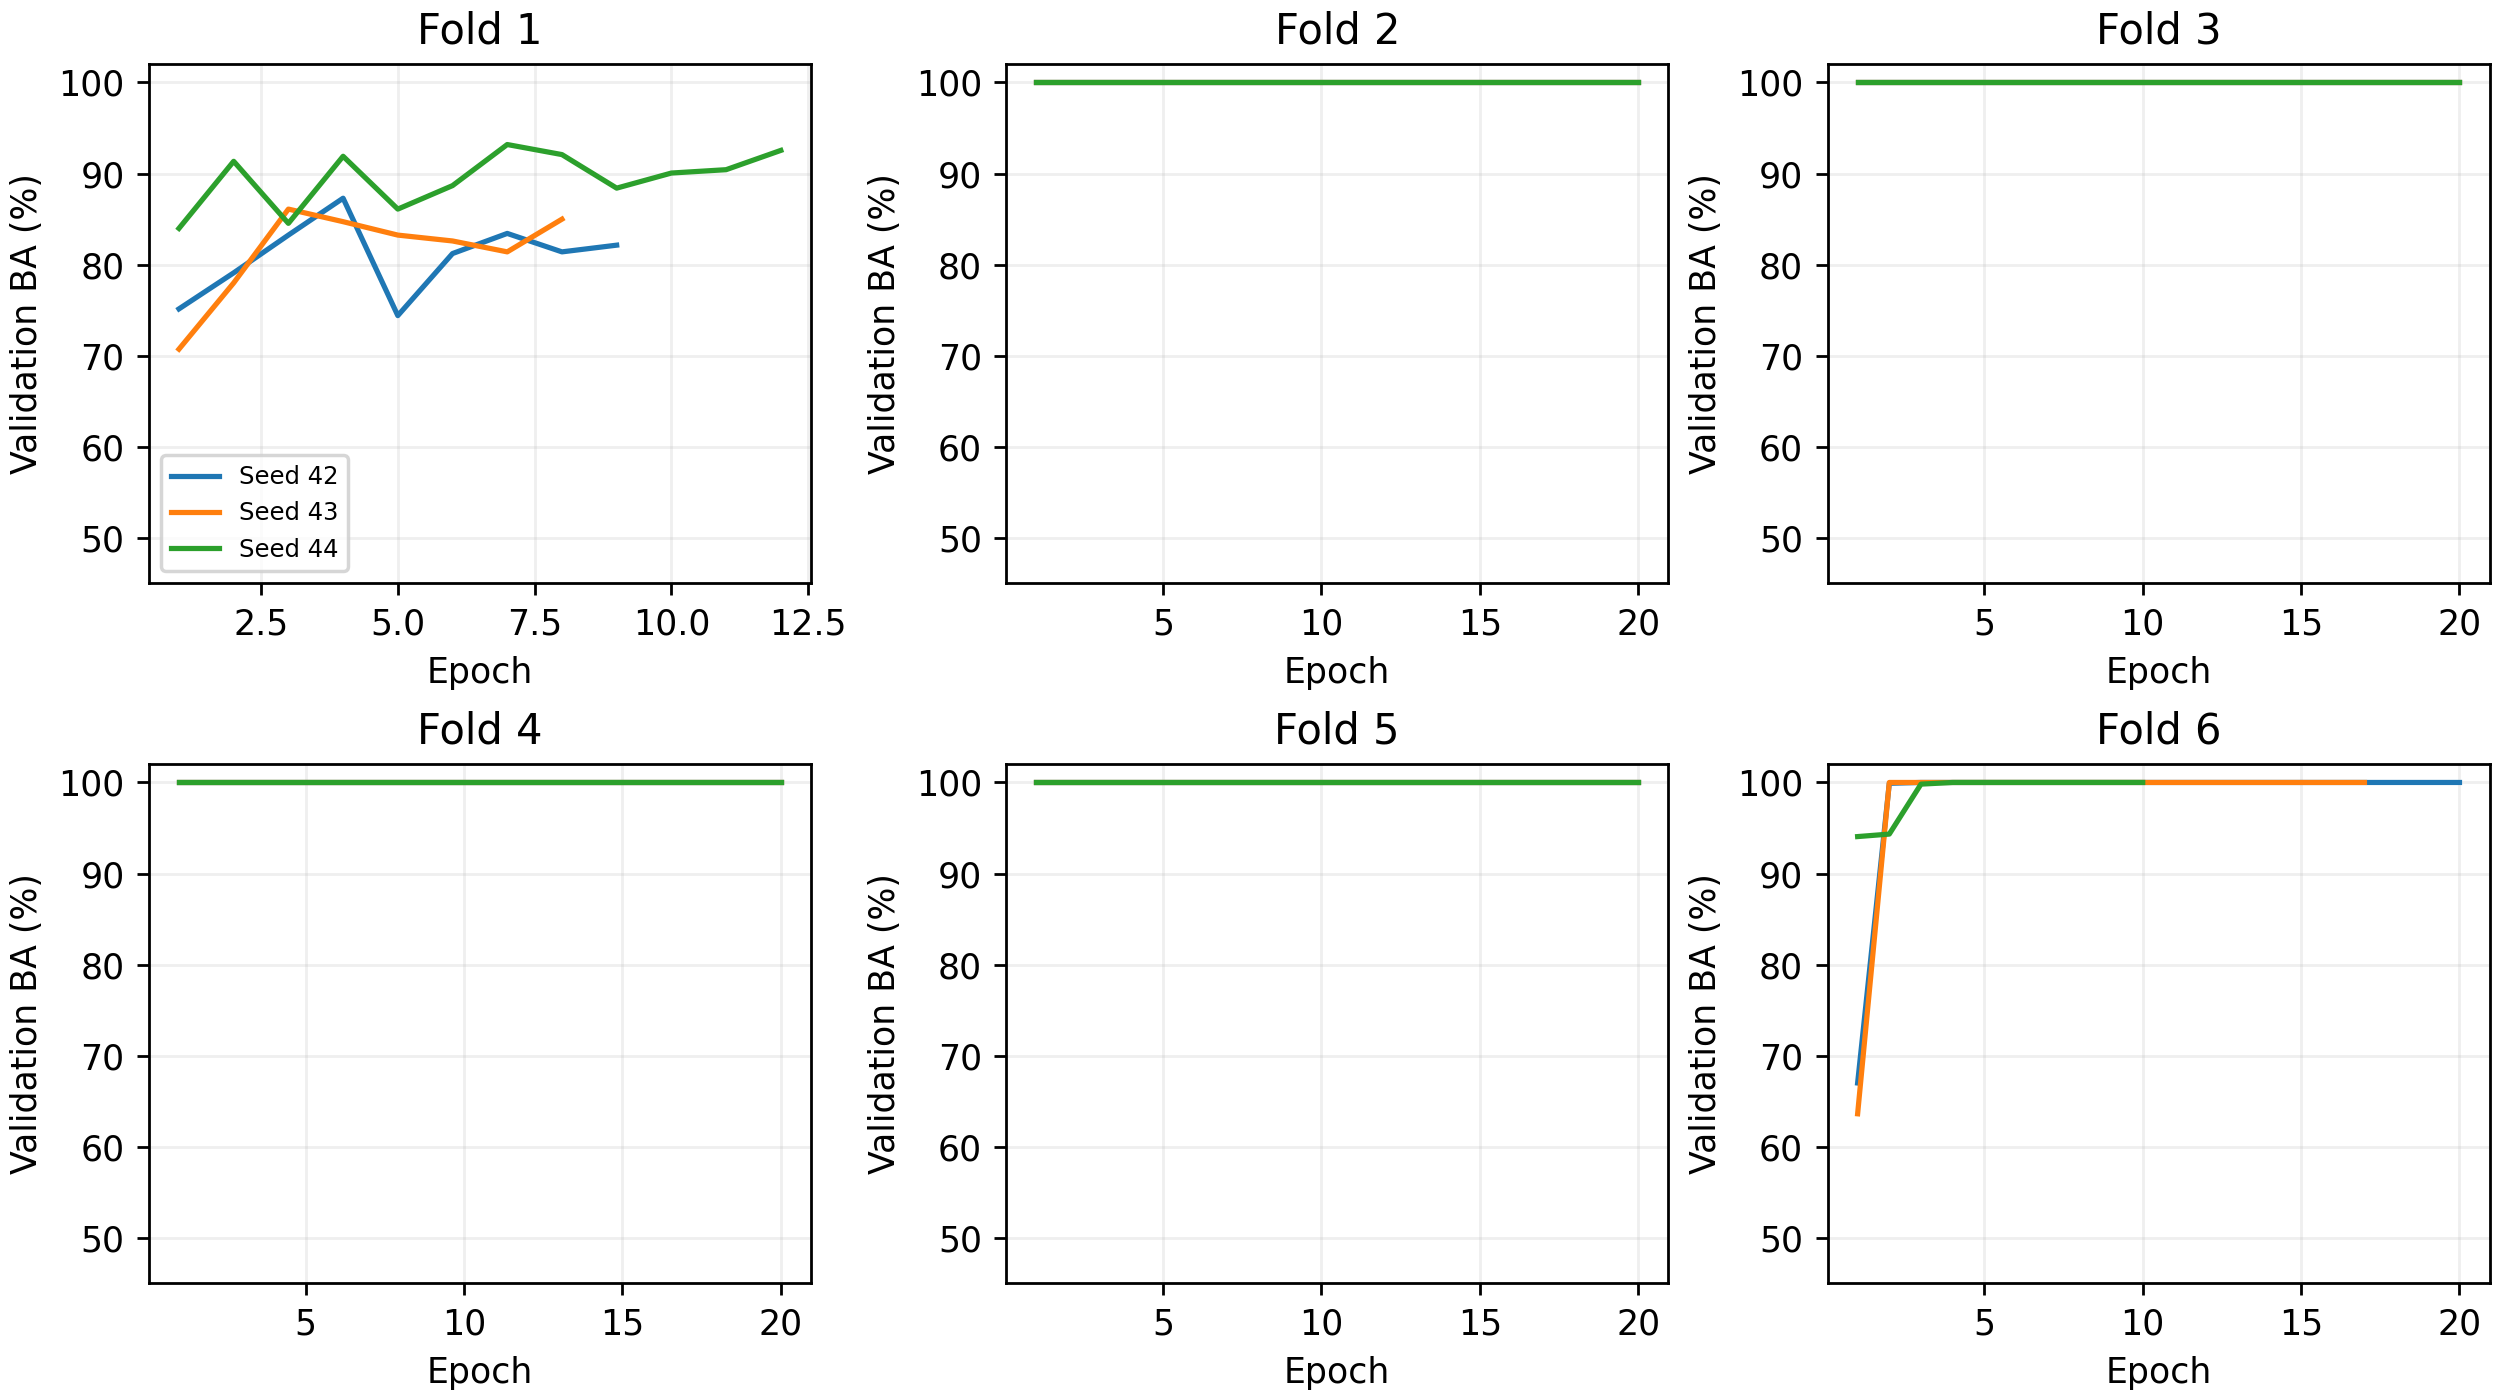
\includegraphics[width=\linewidth,height=0.42\textheight,keepaspectratio]{figures/figure_05.png}
\caption{Validation balanced accuracy over epochs for each source-holdout fold and all three seeds. Curves concern validation only; checkpoint selection does not use test results.}
\label{fig:5}
\end{figure}

\subsection{Controlled additive-noise sensitivity}

\begin{table}[H]
\centering
\caption{Frozen-model additive-noise results, averaged over sources and perturbation/model seeds.}
\label{tab:6}
\footnotesize
\setlength{\tabcolsep}{4pt}
\begin{tabularx}{\linewidth}{@{}YYYYYY@{}}
\toprule
\rowcolor{tablegray}
\textbf{Added SNR dB} & \textbf{DSP recall \%} & \textbf{DSP BA \%} & \textbf{CNN recall \%} & \textbf{CNN BA \%} & \textbf{CNN specificity \%} \\
\midrule
20 & 66.67 & 83.33 & 94.57 & 97.28 & 100.00 \\
15 & 66.67 & 83.33 & 96.14 & 98.07 & 100.00 \\
10 & 66.67 & 83.33 & 94.86 & 94.65 & 94.44 \\
5 & 66.67 & 83.33 & 94.31 & 94.38 & 94.44 \\
0 & 66.74 & 80.59 & 81.09 & 87.77 & 94.44 \\
\bottomrule
\end{tabularx}
\end{table}

Values average source-macro metrics over noise draws and, for CNN, all three model seeds. Clean macro recall/BA are 66.67/83.33\% for DSP and 85.07/92.54\% for CNN. DSP specificity is 100\% at 5-20 dB and 94.44\% at 0 dB. These are descriptive scores on perturbed existing data, including copied backgrounds.

\begin{figure}[H]
\centering
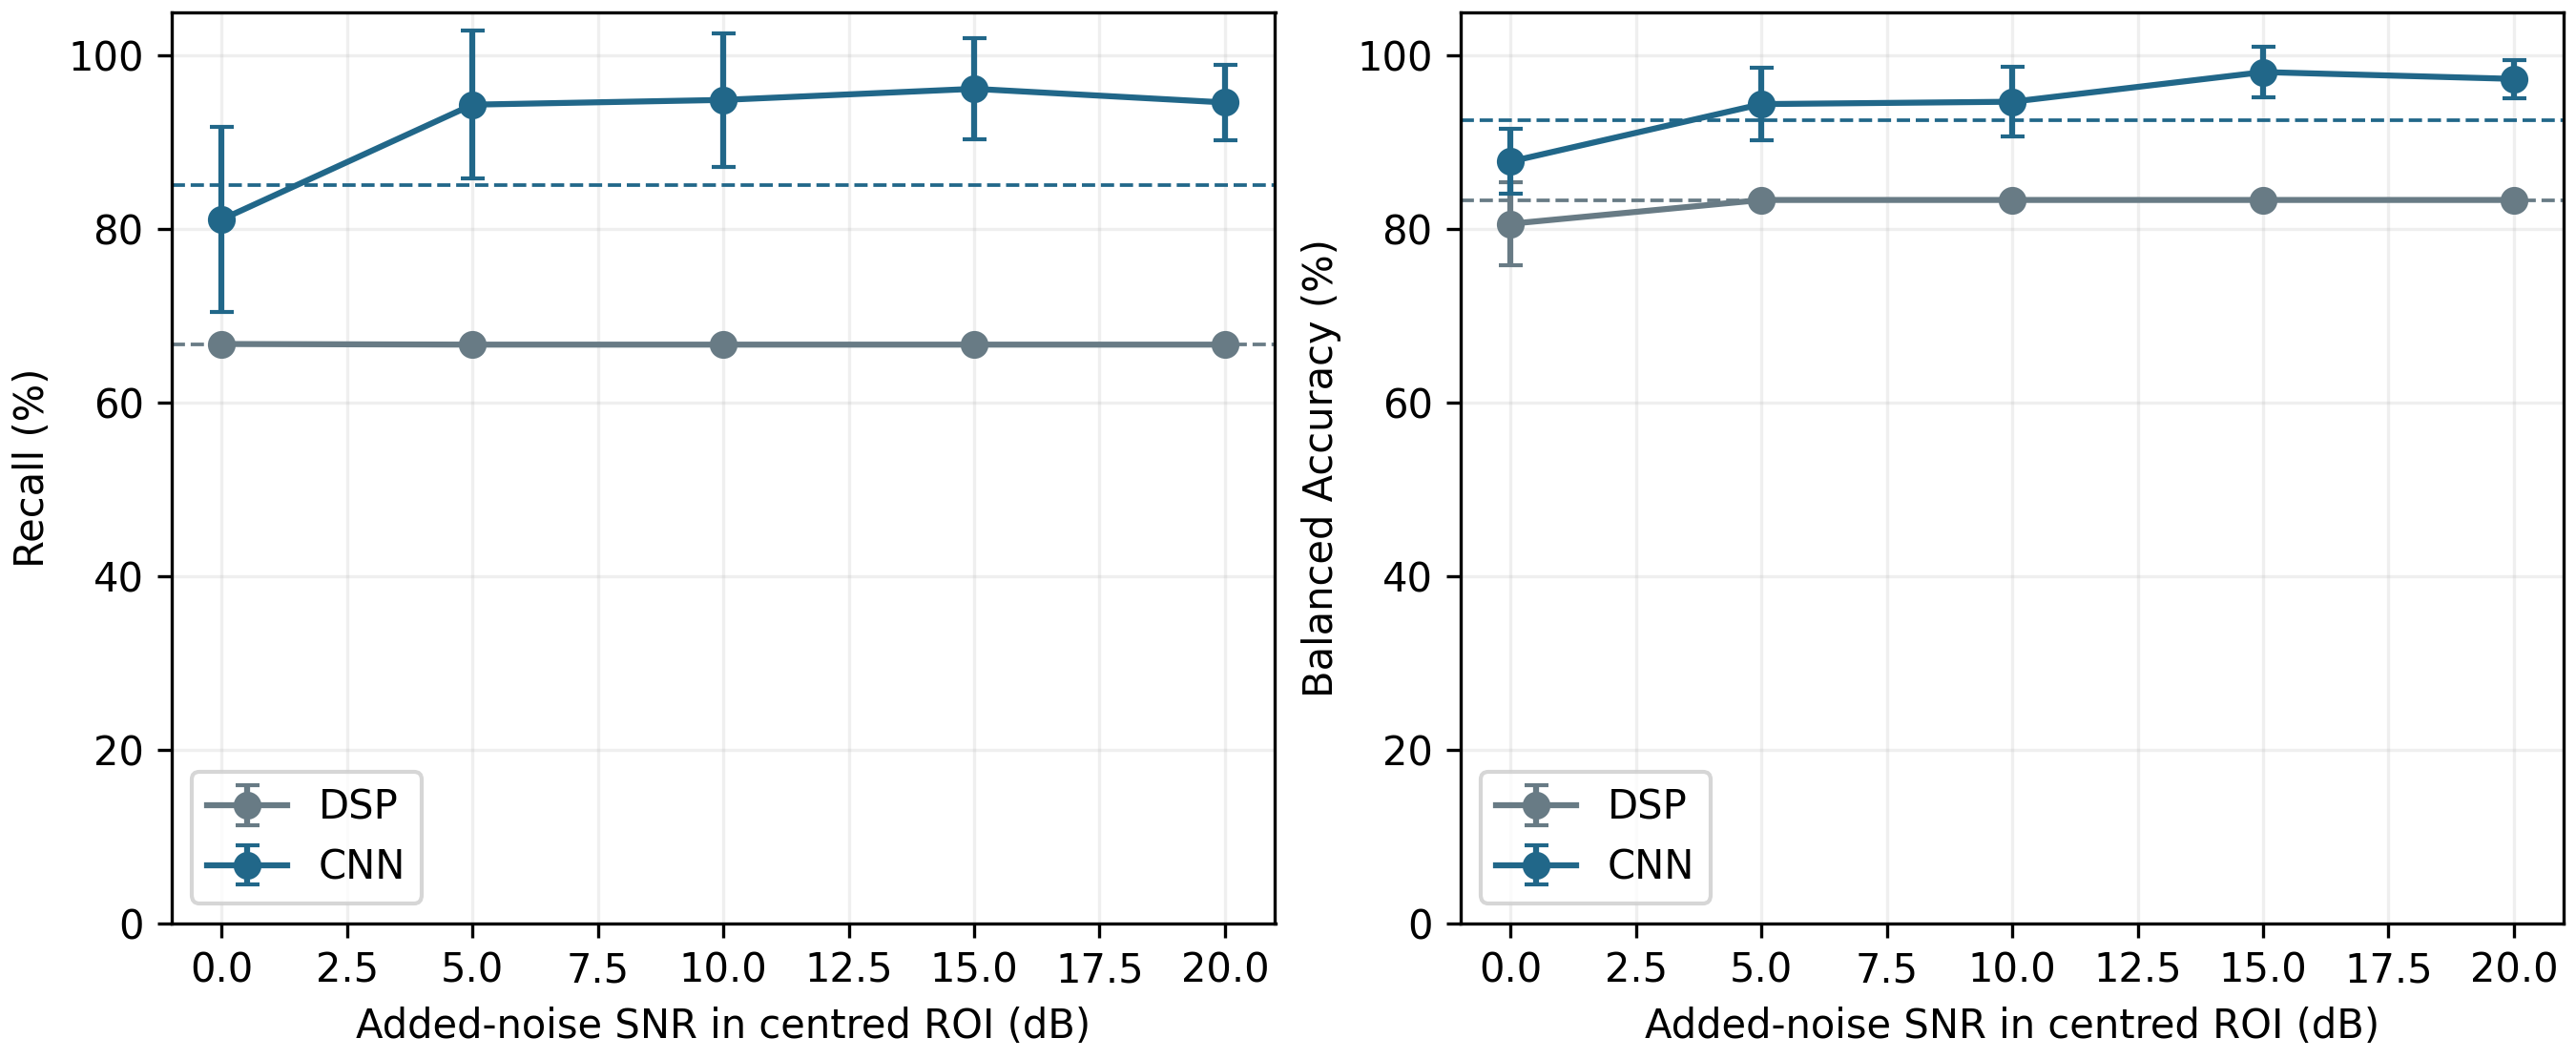
\includegraphics[width=\linewidth,height=0.42\textheight,keepaspectratio]{figures/figure_06.png}
\caption{Frozen-model Gaussian-noise stress test. Error bars are sample SD across noise and model seed combinations; dashed lines mark clean means.}
\label{fig:6}
\end{figure}

The CNN response is nonmonotonic: mean recall rises above its clean value under moderate perturbation, then falls at 0 dB, while false positives appear at 0-10 dB. Added noise changes the envelope and score distribution, sometimes moving previously subthreshold positives across a frozen decision boundary. Increased recall alone is therefore not proof of better robustness. The specificity loss exposes the cost of that movement. Full fold-level results, logits and decisions are saved; no noisy test condition is used to choose a threshold.

\subsection{Simulation-trained transfer on a shared normal background}

\begin{table}[H]
\centering
\caption{Simulation-trained transfer. Target negatives are shared with the training domain.}
\label{tab:7}
\small
\setlength{\tabcolsep}{4pt}
\begin{tabularx}{\linewidth}{@{}YYYYY@{}}
\toprule
\rowcolor{tablegray}
\textbf{Evaluation domain} & \textbf{Method} & \textbf{Recall \%} & \textbf{BA \%} & \textbf{ROC-AUC} \\
\midrule
Simulated reference & DSP & 55.79 & 77.90 & 0.7761 \\
Simulated reference & SVM & 89.48 & 94.74 & 0.9749 \\
Simulated reference & CNN & 72.81 \(\pm\) 3.96 & 86.41 \(\pm\) 1.98 & 0.9778 \\
Experimental target & DSP & 100.00 & 100.00 & 1.0000 \\
Experimental target & SVM & 100.00 & 100.00 & 1.0000 \\
Experimental target & CNN & 100.00 \(\pm\) 0.00 & 100.00 \(\pm\) 0.00 & 1.0000 \\
\bottomrule
\end{tabularx}
\end{table}

CNN values are seed means \(\pm\) sample SD; AUC is the seed mean. Metrics here pool rows within a domain, whereas the primary experiment uses an equal-weight source macro average. They are separate protocols and must not be merged into one model leaderboard.

\begin{figure}[H]
\centering
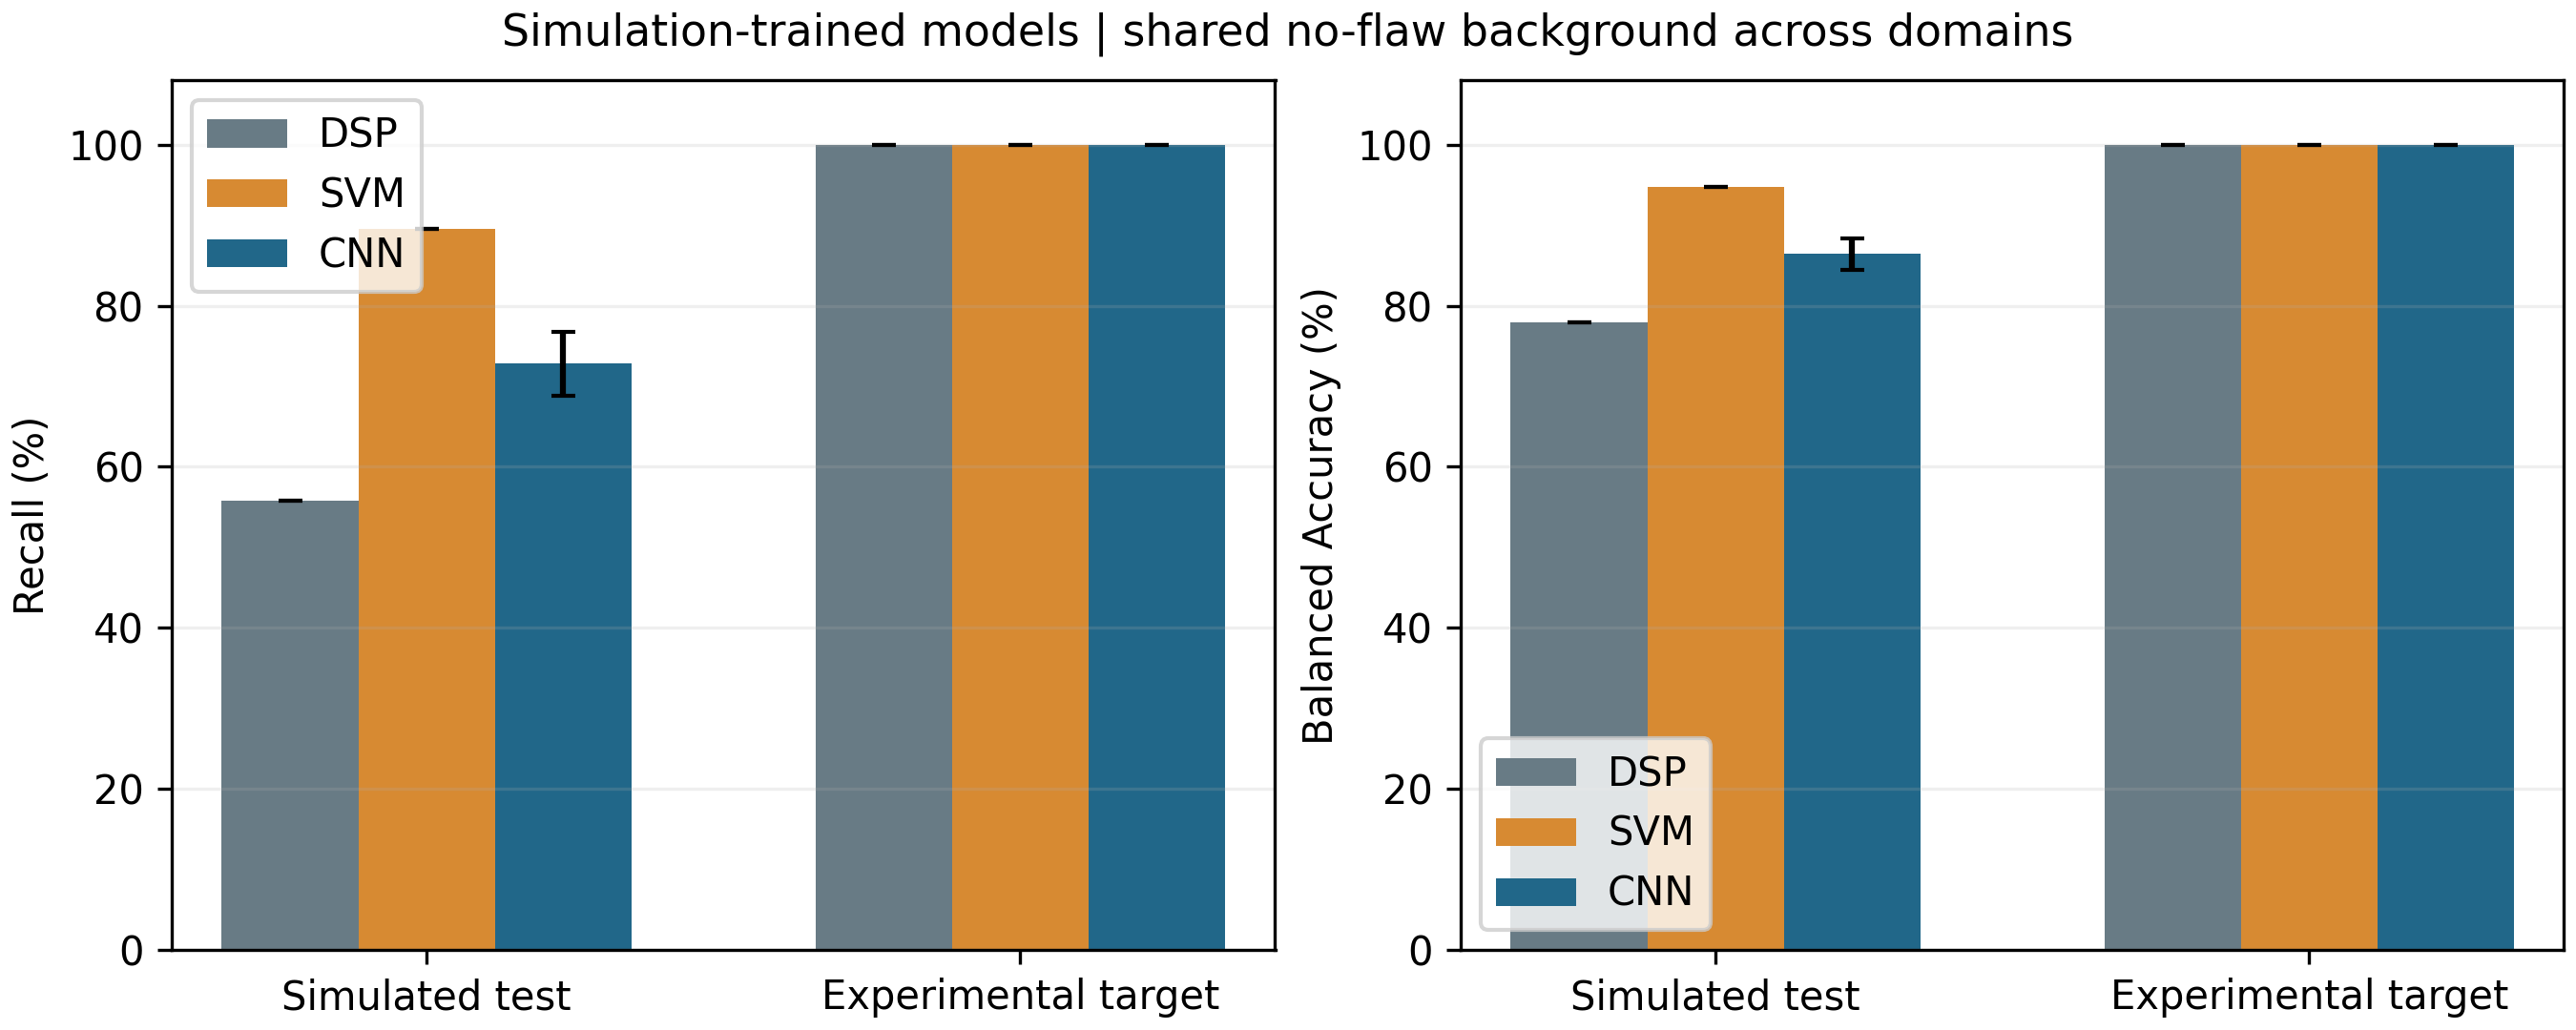
\includegraphics[width=\linewidth,height=0.42\textheight,keepaspectratio]{figures/figure_07.png}
\caption{Simulation-trained models on their untouched simulated test and experimental target. All target negatives also occur in the source domain.}
\label{fig:7}
\end{figure}

All models classify every target positive and negative correctly. However, perfect target specificity is measured on an identical training-domain background, and target positives need not span the same amplitude/difficulty distribution as the simulated reference. The poorer simulated-reference scores show that a dataset labelled experimental is not automatically a harder independent test. The result demonstrates that these frozen simulation-trained decisions transfer to these target rows; it cannot establish deployment performance, a benefit over the original source-holdout models, or general transfer to unseen normal structures.

\subsection{Measured array imaging and nominal-tip discrepancy}

\begin{table}[H]
\centering
\caption{Measured TFM peaks and distance to the approximate nominal lower tip.}
\label{tab:8}
\small
\setlength{\tabcolsep}{4pt}
\begin{tabularx}{\linewidth}{@{}YYY@{}}
\toprule
\rowcolor{tablegray}
\textbf{Reconstruction} & \textbf{ROI peak x, depth mm} & \textbf{Distance to nominal tip mm} \\
\midrule
Initial t0=0 & 29.25, 18.50 & 5.94 \\
Backwall-calibrated & 37.50, 17.00 & 3.91 \\
\bottomrule
\end{tabularx}
\end{table}

\begin{figure}[H]
\centering
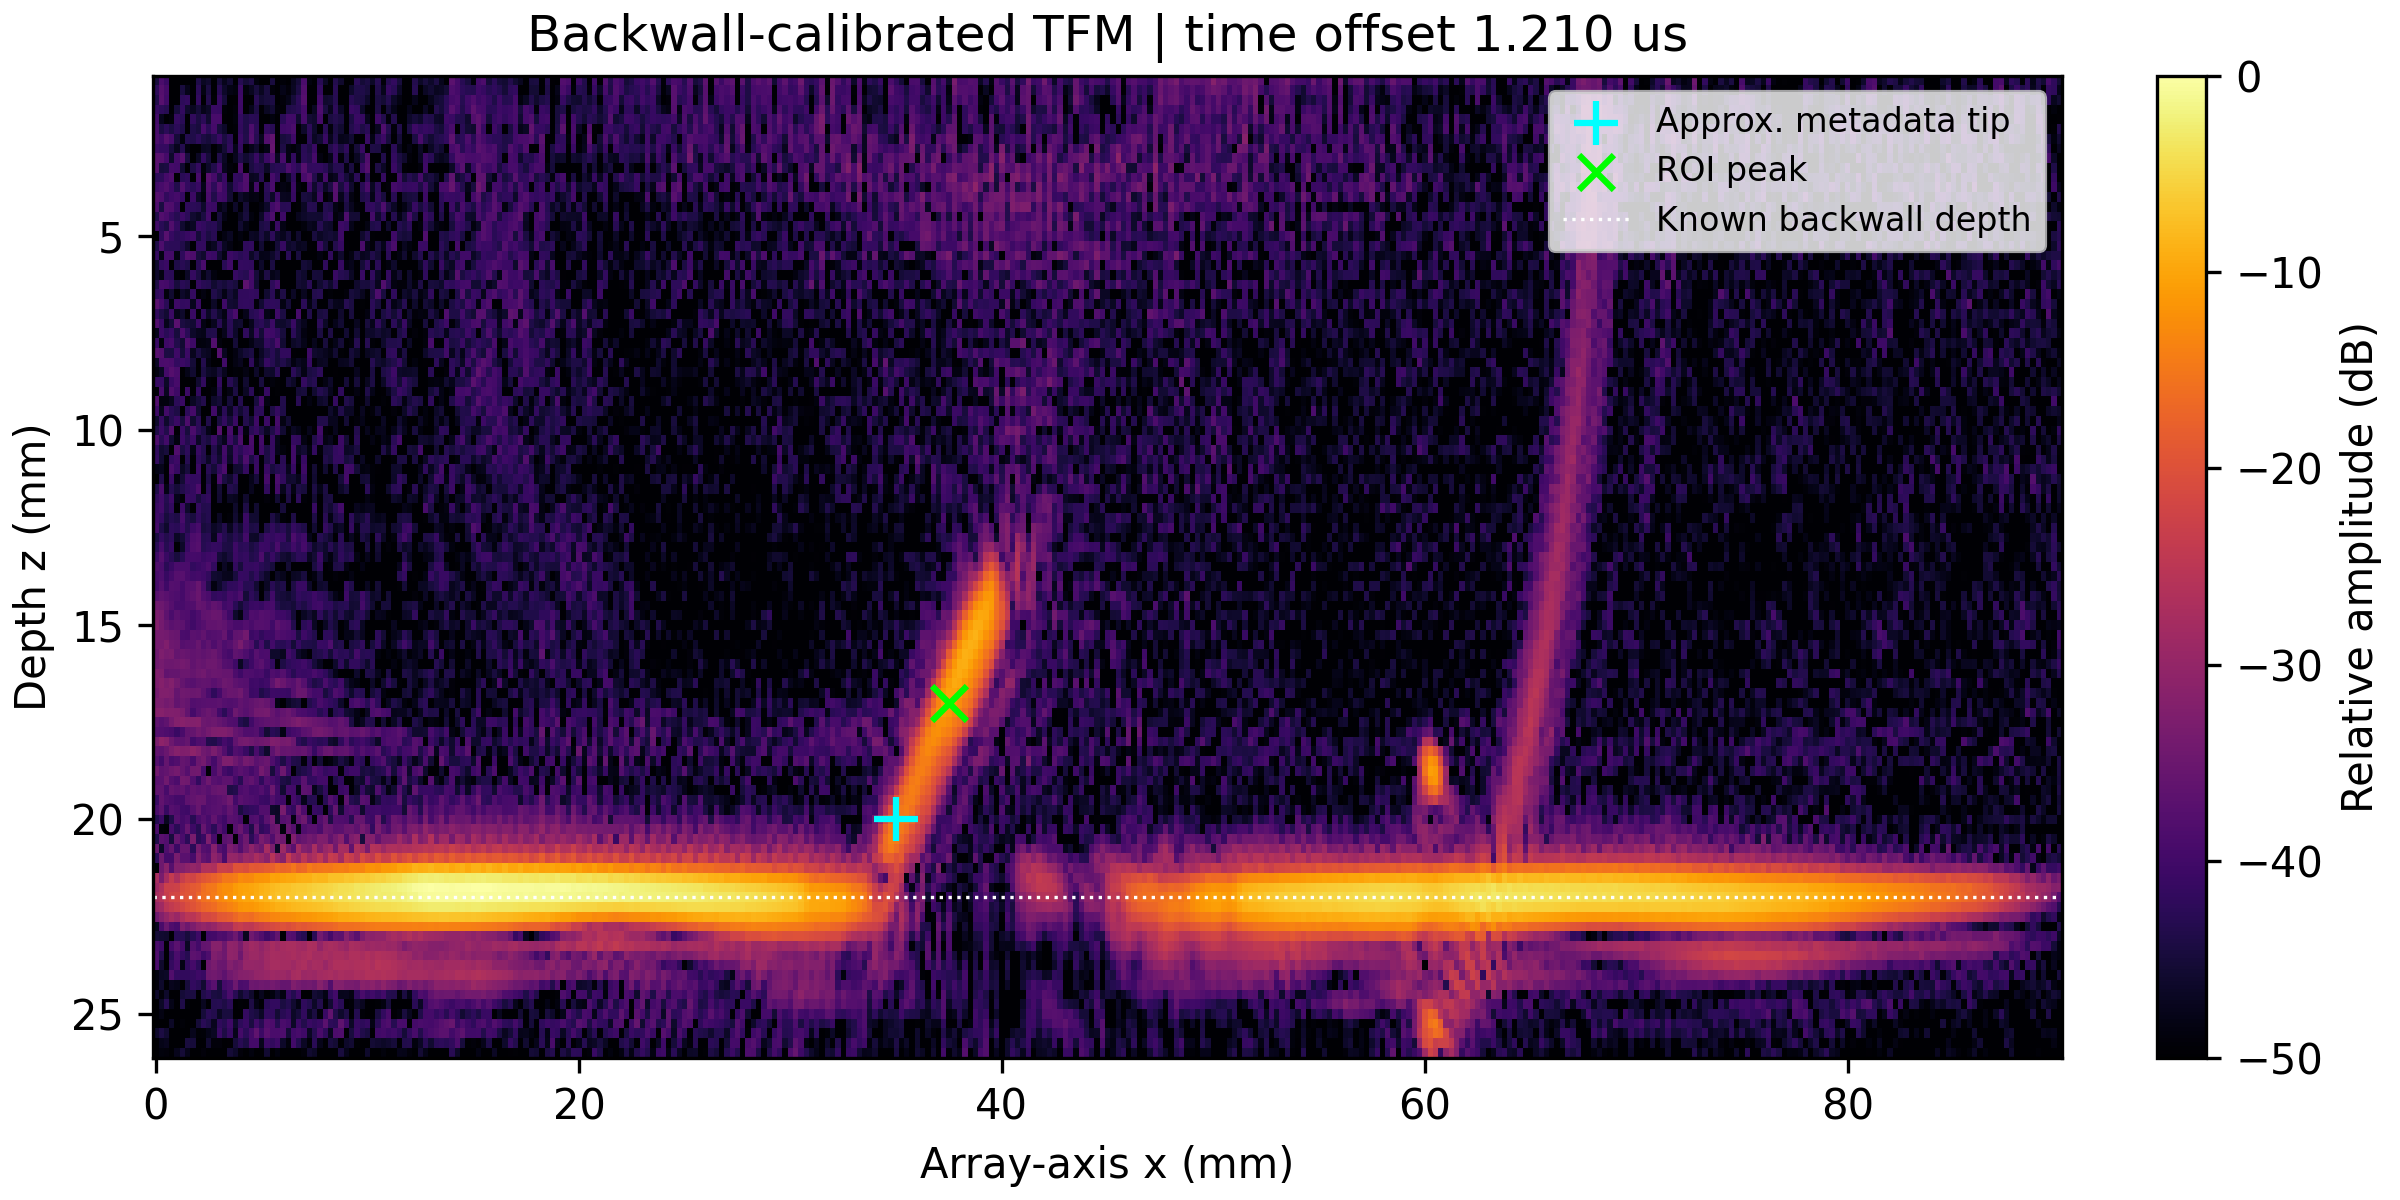
\includegraphics[width=\linewidth,height=0.42\textheight,keepaspectratio]{figures/figure_08.png}
\caption{Backwall-calibrated TFM from measured welded-plate FMC data. The cyan reference is approximate; the bright ROI peak is not a verified crack tip.}
\label{fig:8}
\end{figure}

Backwall calibration reduces the nominal-point discrepancy, but the calibrated peak is on the upper boundary of the search ROI. That behaviour indicates an unreliable tip assignment, not successful accurate localisation. The 0.25 mm grid spacing is numerical sampling, not achieved physical resolution or measurement accuracy. Both images, calibration arrivals, reconstruction grids and error calculations are included. The imaging pilot is implemented and numerically checked, with a negative result for dependable crack-tip identification under this simplified model.

\FloatBarrier
\section{Discussion}

\subsection{Answering the research question}

The CNN improves macro recall by 18.40 percentage points over the frozen DSP detector, but is 14.72 points below the SVM. On the 2 mm source, seeds 42, 43 and 44 detect only 60, 22 and 89 of 547 positive rows, respectively; the SVM detects 540. All CNN source-holdout ROC-AUC values are 1.0 despite this weak 2 mm recall. Thus a learned ranking can still transfer better than its fixed operating point, just as with the DSP score. The CNN is not the best-performing method here, and the result does not justify replacing the SVM. No threshold is adjusted after observing this result.

The comparison tests a specific operating pipeline: shared DSP preprocessing followed by either a frozen amplitude decision rule or a small convolutional classifier. Improvement should therefore be interpreted relative to that detector, not as proof that convolution is universally superior to DSP. The SVM reference is important because it already resolves much of the threshold-transfer failure using a compact engineered representation. The tables identify whether the CNN adds anything beyond that reference.

The saved DSP ROC-AUC remains 1.0 in every evaluation despite zero recall for the two smallest held-out sources. Its validation threshold is effectively constrained by the validation source's amplitude range; a smaller test-source response can remain above all negatives but below that threshold. This is a calibration/operating-point failure rather than loss of ranking. A learned rule can exploit additional spatial or amplitude relationships, but a CNN's fixed 0.5 score threshold can also fail under source shift. The experiment does not identify a causal explanation for every error without an additional ablation.

The fold composition gives a concrete interpretation of the small-source asymmetry. Fold 1 excludes both the 2 mm test source and the 3 mm validation source from training; its four training source labels have nominal sizes of 6 mm or larger. Fold 2, by contrast, includes the 2 mm source in training when testing the 3 mm source. This is consistent with difficult downward transfer in source size, but it does not isolate size causally: reflector type, augmentation and response amplitude also differ.

\subsection{Unequal model development budgets}

The SVM underwent a validation search over 25 configurations: five linear C values and 20 RBF C/gamma combinations. The CNN used one architecture and optimizer configuration, repeated across three seeds. Seeds explore training variability, not alternative architectures or learning rates. Therefore, the SVM had a broader configuration-selection opportunity, while the CNN had repeated initializations. This comparison ranks the saved pipelines under their actual development budgets; it does not establish that SVMs intrinsically outperform CNNs or that a fairly optimized CNN would necessarily improve.

There is also an operating-rule difference. DSP selects its threshold on validation rows, whereas the CNN fixes a sigmoid threshold of 0.5 and uses validation for checkpoint selection. Shared test samples make the outcome comparison controlled, but do not make model-selection procedures identical. A stronger follow-up would assign comparable validation-search budgets and predefine threshold selection for each method, then evaluate on fresh held-out acquisitions. Choosing a new threshold from the test-score gap in Figure~\ref{fig:4} would invalidate the current test as an untouched assessment.

\subsection{Relationship to published work}

The poor 2 mm recall is directionally consistent with Koskinen et al.'s observation that training on larger indications can leave smaller unseen flaws difficult \cite{ref2}. This report adds a different diagnostic: the saved logits still rank that source perfectly, so failure at the frozen boundary is demonstrably different from an inability to order the examples. This does not identify which learned features caused the score shift. A feature or normalization ablation would be needed for that causal claim.

The context-aware and sound-data approaches \cite{ref5,ref6} suggest distinct follow-up questions: whether additional acquisition context changes the decision boundary, and whether diverse sound acquisitions support an anomaly detector. Neither can be evaluated convincingly by recycling the single repeated negative image. The present results therefore complement these research directions through a data-quality and operating-point diagnosis; they neither reproduce nor contradict their published performance.

\subsection{What the comparison does and does not isolate}

Keeping the raw samples, ROI and fold manifests fixed reduces obvious confounding from different datasets or easier test partitions. However, the CNN also changes representation through block pooling and log compression. A performance difference cannot be assigned solely to convolutional architecture, since these representation choices are not ablated. Useful follow-up comparisons would include an MLP on the same maps, a CNN without compression, and validation-selected CNN thresholds. Such experiments should be designed on fresh development data rather than adapted after observing these test results.

Three seeds make initialization sensitivity visible but are not independent physical experiments. Reporting all seeds avoids choosing a favourable test run; it does not establish a confidence interval for future flaws. Likewise, the six source labels are a limited and related set. Mean performance across them is descriptive and should not be assigned a broad population interpretation or an unsupported significance claim.

\subsection{Principal limitations and how to resolve them}

The repeated negative background is the strongest limitation. A model can recognize that background consistently while remaining untested on different couplings, materials, clutter or instruments. Consequently, specificity and false-positive counts must be read as performance on one repeated background. Resolving this requires independently acquired negative specimens and acquisition-group splits.

Distinct positive hashes do not eliminate augmentation dependence. Grouping by source label reduces direct source reuse across positive partitions, but cannot establish new-specimen independence. More original cracks and acquisition metadata would permit a stronger specimen-level evaluation. In particular, a binomial confidence interval treating every augmented row as independent would overstate precision and is not reported.

The map representation trades resolution for tractability. Narrow echoes can be retained by maximum pooling while subtle spatial texture is lost; global pooling also removes explicit location. Neither depth nor scan-axis localisation is inferred by the CNN. The separate measured-FMC pilot implements imaging but does not achieve reliable tip identification. The noise study is a controlled synthetic perturbation rather than a substitute for new acquisitions. Independent-background evaluation and a preplanned representation ablation remain necessary to broaden the binary-detection conclusion.

\subsection{What the supplementary tests add}

The noise study reinforces the operating-point diagnosis: input perturbation can increase recall and simultaneously introduce false alarms, so a monotonic degradation assumption would be misleading. Synthetic Gaussian noise is useful because its strength is controlled, but limited because real inspection changes are structured and may alter signal propagation. Paired noise fields and duplicate-aware assignment avoid presenting copied negatives as new independent acquisitions.

The transfer audit is as consequential as its perfect target scores. A background shared between simulation and experiment weakens the claim of a domain shift precisely where false-positive reliability matters. No target positive image is byte-identical to a simulated positive, but this rules out only exact identity. It does not establish unrelated physical sources. The appropriate conclusion is narrow positive-response transfer under a shared-background condition, with independent normal acquisitions still required.

The imaging pilot exposes a separate physics limit: delay-and-sum code can pass a point-target test and produce a plausible measured image while failing to identify the intended crack tip. Backwall calibration removes one global timing discrepancy; it cannot correct spatially varying weld velocities or distinguish tip diffraction from other bright responses. A boundary maximum and approximate reference point prohibit an accuracy claim. A subsequent validated study would need independent geometric truth and an appropriate propagation model. These observations support the report's emphasis on evaluation conditions rather than headline scores.

\FloatBarrier
\section{Conclusion}

For this dataset and the frozen source-holdout protocol, adding the compact CNN improves macro recall over the deterministic detector by 18.40 percentage points, chiefly by recovering the 3 mm source. It does not outperform the saved engineered-feature SVM, and its mean 2 mm recall remains only 10.42\%. Figure~\ref{fig:4} establishes that ranking and the fixed operating boundary transfer differently even within the CNN pipeline.

The contribution is the controlled comparison and its diagnosis, not a superior CNN architecture. Source-wise reporting and image-identity auditing reveal weaknesses hidden by perfect ordinary-split accuracy. The question is answered for these six source labels and actual development budgets; independent-background specificity and new-specimen generalisation remain unestablished. The completed supplementary studies demonstrate nonmonotonic frozen-threshold noise sensitivity, perfect but shared-background simulation-trained transfer, and an implemented measured-FMC reconstruction with unreliable tip identification. Broader conclusions require new acquisitions, comparable model-selection budgets and predefined threshold handling rather than further tuning against these test results.

\FloatBarrier
\section{Reproducibility and references}

The repository includes working inference code, fixed demonstration inputs, all selected weights, split manifests, per-sample predictions, training curves and numerical verification. Run \texttt{python src/demo\_cnn.py} for the portable demonstration and \texttt{python src/verify\_cnn\_results.py} to check the saved experiment without fitting a model. \texttt{requirements-cnn.txt} records the final-stage environment. Raw data and the large local cache are excluded; the original upstream dataset is linked in the README. Full training instructions and the fixed protocol are documented separately. The report and video are linked from the repository. Supplementary working code and raw-data reproduction instructions are in \path{docs/methodology/completed_extensions.md}. Run \texttt{python src/verify\_extensions.py} to check all saved extension results without raw data or model fitting. Raw FMC and simulated streams are excluded. Public dataset provenance and the CC BY 4.0 attribution are retained.

AI assistance: OpenAI Codex assisted with implementation, experiment orchestration, verification and report preparation. The cited publications and upstream dataset are credited below; the author retains responsibility for the submitted analysis.

\FloatBarrier

\begingroup\small\setlength{\parskip}{0pt}

\begin{thebibliography}{8}

\addcontentsline{toc}{subsection}{References}

\bibitem{ref1} I. Virkkunen, T. Koskinen, O. Jessen-Juhler and J. Rinta-aho, ``Augmented Ultrasonic Data for Machine Learning,'' Journal of Nondestructive Evaluation, vol. 40, art. 4, 2021. \url{https://doi.org/10.1007/s10921-020-00739-5}

\bibitem{ref2} T. Koskinen, I. Virkkunen, O. Siljama and O. Jessen-Juhler, ``The Effect of Different Flaw Data to Machine Learning Powered Ultrasonic Inspection,'' Journal of Nondestructive Evaluation, vol. 40, art. 24, 2021. \url{https://doi.org/10.1007/s10921-021-00757-x}

\bibitem{ref3} C. Cortes and V. Vapnik, ``Support-vector networks,'' Machine Learning, vol. 20, pp. 273-297, 1995. \url{https://doi.org/10.1007/BF00994018}

\bibitem{ref4} Y. LeCun, L. Bottou, Y. Bengio and P. Haffner, ``Gradient-based learning applied to document recognition,'' Proceedings of the IEEE, vol. 86, no. 11, pp. 2278-2324, 1998. \url{https://doi.org/10.1109/5.726791}

\bibitem{ref5} H. Herve-Cote, F. Dupont-Marillia and P. Belanger, ``Automatic flaw detection in sectoral scans using machine learning,'' Ultrasonics, vol. 141, art. 107316, 2024. \url{https://doi.org/10.1016/j.ultras.2024.107316}

\bibitem{ref6} S. McKnight, V. Tunukovic, A. Hifi, S. G. Pierce, E. Mohseni, C. N. MacLeod and T. O'Hare, ``Three-dimensional ultrasonic self supervised segmentation,'' Engineering Applications of Artificial Intelligence, vol. 154, art. 110870, 2025. \url{https://doi.org/10.1016/j.engappai.2025.110870}

\bibitem{ref7} T. Lardner (creator) and K. M. M. Tant (contributor), ``FMC dataset,'' University of Strathclyde, 2015, dataset and acquisition metadata, CC BY 4.0. \url{https://doi.org/10.15129/a7da5071-0436-4913-8f0e-de78f5ebccd6}

\bibitem{ref8} C. Holmes, B. W. Drinkwater and P. D. Wilcox, ``Post-processing of the full matrix of ultrasonic transmit-receive array data for non-destructive evaluation,'' NDT \& E International, vol. 38, no. 8, pp. 701-711, 2005. \url{https://doi.org/10.1016/j.ndteint.2005.04.002}

\end{thebibliography}\endgroup
\end{document}
